\documentclass{scrartcl}

\usepackage{fixltx2e}

% Step environment
% <https://tex.stackexchange.com/a/12943/13262>
\usepackage{amsthm}
\newtheorem*{remark}{Remark}
%
\newtheoremstyle{named}{}{}{\itshape}{}{\bfseries}{.}{.5em}{\thmnote{#1 }#3}
\theoremstyle{named}
\newtheorem*{step}{Step}

\usepackage{microtype}
\usepackage{amsmath}
\usepackage{mathtools}
\usepackage{booktabs}
\usepackage{tabularx}

\usepackage{pgfplots}
\pgfplotsset{compat=newest}

\usepackage{siunitx}

\newcommand\mytitle{How to evaluate and optimize color spaces against experimental data}
\newcommand\myauthor{Nico Schlömer}

\usepackage[
  pdfencoding=unicode,
  ]{hyperref}
\hypersetup{
  pdfauthor={\myauthor},
  pdftitle={\mytitle}
}

% <https://tex.stackexchange.com/a/43009/13262>
\DeclarePairedDelimiter\abs{\lvert}{\rvert}%
\DeclarePairedDelimiter{\norm}{\lVert}{\rVert}

\usepackage[T1]{fontenc}
\usepackage{newtxtext}
\usepackage{newtxmath}

% degree symbol
\usepackage{gensymb}

% % <https://tex.stackexchange.com/a/413899/13262>
% \usepackage{etoolbox}
% \makeatletter
% \long\def\etb@listitem#1#2{%
%   \expandafter\ifblank\expandafter{\@gobble#2}
%     {}
%     {\expandafter\etb@listitem@i
%      \expandafter{\@secondoftwo#2}{#1}}}
% \long\def\etb@listitem@i#1#2{#2{#1}}
% \makeatother

% Okay. Don't use biblatex/biber for now. There are breaking changes in every
% revision, and we'd have to stick to the exact version that arxiv.org has,
% otherwise it's error messages like
% ```
% Package biblatex Warning: File 'main.bbl' is wrong format version
% - expected 2.8.
% ```
% \usepackage[sorting=none]{biblatex}
% \bibliography{bib}

\usepackage{amsmath}
\DeclareMathOperator{\sign}{sign}
\DeclareMathOperator*{\argmin}{arg\,min}

% \usepackage{amsfonts}
\usepackage{bm}
\newcommand\rr{\ensuremath{\bm{r}}}
\newcommand\R{\ensuremath{\mathbb{R}}}
\newcommand\xt{\ensuremath{\bm{\tilde{x}}}}
\newcommand\yt{\ensuremath{\bm{\tilde{y}}}}

\title{\mytitle\footnote{The LaTeX sources of this article are on
\url{https://github.com/nschloe/colorio}}}
\author{\myauthor}

\begin{document}

\maketitle
\begin{abstract}
  todo
\end{abstract}

\section{Introduction}

Every year, articles on new color spaces are created, claiming that they comply to
certain experimental data better than other color spaces. In many cases, numbers are
provided in form of a table showing that the new color space is indeed better.
Unfortunately, it is hardly ever explained how those numbers are computed.

This article describes in detail how to assess the experimental compliance of color
space with experimental data. The article focuses on the two most used types of
experimental data: Hue linearity \cite{ebner,xiao,hung} and color difference ellipses
\cite{macadam1942,luorigg}.

Almost every color space is defined by a transformation $T$ that maps the CIE-1931-XYZ
coordinates into a three-dimensional new coordinate space (e.g., LAB). The
transformation is usually continuously differentiable and bijective. When talking about
a colorspace, one almost always means the transformation $T$ and its inverse.


TODO desirable properties of cost functionals:
\begin{itemize}
  \item Are continuous, and ideally continuously differentiable (for optimization)
  \item Are 0 if the experimental data is matched exactly (will never be fulfilled since
    experimental data contains errors). Together with the first one, number are small if
    the match is approximate.
  \item are scaling invariant
  \item are rotation invariant
  \item are translation invariant
\end{itemize}


\section{Average, root mean square, and how to combine results}

In several stages of the assessment or optimization process, we will have to combine
several positive result values (e.g., residuals from different data sets) into one.
There are multiple meaningful ways of doing so. The most common are certainly the
\emph{average} and the \emph{root mean square} of different results
$\rr = \{|r_i|\}_{i=1}^n$,
\[
  M_1(\rr) = \frac{1}{n}\sum_{i=1}^n r_i,\quad
  M_2(\rr) = \sqrt{\frac{1}{n}\sum_{i=1}^n r_i^2}.
\]
This is readily generalized to the
\emph{generalized mean}
\[
  M_p(\rr) \coloneqq \left(\frac{1}{n}\sum_{i=1}^n r_i^p\right)^{1/p} =
  \frac{1}{n^{1/p}} \|\rr\|_p
\]
with any given $-\infty \le p \le \infty$. In the limits, $p\to-\infty$, $p\to 0$ and
$p\to +\infty$, this becomes the \emph{minimum}, the \emph{geometric mean}, and the
\emph{maximum}
\[
  M_{-\infty}(\rr) \coloneqq \min_{i\in\{1,\dots,n\}} r_i, \quad
  M_0(\rr) \coloneqq \left(\prod_{i=1}^n r_i\right)^{1/n}, \quad
  M_{\infty}(\rr) \coloneqq \max_{i\in\{1,\dots,n\}} r_i.
\]
Note that, for every $\rr$, $M_p(\rr)$ as a function in $p$ is smooth and monotonic
increasing
\[
  M_{-\infty}(\rr) \le M_p(\rr) \le M_q(\rr) \le M_{\infty}(\rr) \quad (p\le q).
\]
(Compare figure \ref{fig:1}.)
Hence, the larger $p$, the closer $M_p(\rr)$ will be to $\max(\rr)$.
This makes a larger $p$ suitable, for example, for an optimization process that tries to
minimize the maximum STRESS (see section~\ref{}).

Choosing $p < 1$, on the other hand, puts more emphasis on the smaller values in $\rr$.
In particular, $M_0(\rr)=0$ if only one $r_i=0$. One almost never wants this in the
context of experimental validation or optimization.

\begin{figure}
  \centering
  % This file was created by tikzplotlib v0.9.9.
\begin{tikzpicture}

\definecolor{color0}{rgb}{0.12156862745098,0.466666666666667,0.705882352941177}
\definecolor{color1}{rgb}{1,0.498039215686275,0.0549019607843137}
\definecolor{color2}{rgb}{0.172549019607843,0.627450980392157,0.172549019607843}
\definecolor{color3}{rgb}{0.83921568627451,0.152941176470588,0.156862745098039}
\definecolor{color4}{rgb}{0.580392156862745,0.403921568627451,0.741176470588235}

\begin{axis}[
axis line style={white!58.8235294117647!black},
height=0.4\textwidth,
legend cell align={left},
legend style={
  fill opacity=0.8,
  draw opacity=1,
  text opacity=1,
  at={(0.09,0.5)},
  anchor=west,
  draw=white!80!black
},
tick align=outside,
tick pos=left,
width=\textwidth,
x grid style={white!58.8235294117647!black},
xlabel={\(p\)},
xmin=-5, xmax=5,
xtick style={color=white!58.8235294117647!black},
y grid style={white!58.8235294117647!black},
ymajorgrids,
ymin=-0.05, ymax=1.1,
ytick style={color=white!58.8235294117647!black}
]
\addplot [semithick, color0]
table [search path=figures/] {averages-000.tsv};
\addlegendentry{\(s_{equal1}\)}
\addplot [semithick, color1]
table [search path=figures/] {averages-001.tsv};
\addlegendentry{\(s_{outlier-small}\)}
\addplot [semithick, color2]
table [search path=figures/] {averages-002.tsv};
\addlegendentry{\(s_{uniform}\)}
\addplot [semithick, color3]
table [search path=figures/] {averages-003.tsv};
\addlegendentry{\(s_{outlier1}\)}
\addplot [semithick, color4]
table [search path=figures/] {averages-004.tsv};
\addlegendentry{\(s_{equal0}\)}
\end{axis}

\end{tikzpicture}

  \caption{$p$-means for sequences of length $n=20$, $s_\text{equal1} = \{1, \dots,
  1\}$, $s_\text{outliner-small} = \{10^{-4}, 1,\dots, 1\}$, $s_\text{uniform} =
  \{10^{-4}, h, 2h, \dots, 1\}$ (with $h = 1 / (n-1)$), $s_\text{outlier1} = \{1,
  0,\dots, 0\}$, and $s_\text{equal0} = \{0,\dots,0\}$. Note how the $M_p$ are monotonic
  increasing and smooth. For large $p$, all curves approach the maximum value in the
  set.}
  \label{fig:1}
\end{figure}


\section{Residuals and STRESS}

% There are numerous experiments~\cite{ebner,xiao,hung,macadam,macadam,luo} which try to
% gauge perceptual distances between colors or to determine which colors of different
% luminosity are perceived as the same chroma.
%
% These experimental data have been used in the past to approximate a perceptually uniform
% colorspace, i.e., a color space in which the Euclidean distance represents the perceived
% distance, and in which colors of same chroma all sit in one line. (These two goals are
% mutually inclusive.) So far, the general approach was to assume that the transformation
% from XYZ space takes a certain mathematical form with a number of free parameters, e.g.,
% the parameters $e$, $\alpha_{i,j}$, and $\omega_{i,j}$.
% \begin{equation}\label{eq:safdar}
%   \begin{split}
%     \begin{bmatrix}
%       L\\M\\S
%     \end{bmatrix}
%     =
%     \begin{bmatrix}
%       \alpha_{1,1} & \alpha_{1,2} & 1 - \alpha_{1,1} - \alpha_{1,2}\\
%       \alpha_{2,1} & \alpha_{2,2} & 1 - \alpha_{2,1} - \alpha_{2,2}\\
%       \alpha_{3,1} & \alpha_{3,2} & 1 - \alpha_{3,1} - \alpha_{3,2}
%     \end{bmatrix}
%     \begin{bmatrix}
%       X_{D65}\\Y_{D65}\\Z_{D65}
%     \end{bmatrix}\\
%     \{L',M',S'\} = \left(\frac{c_1 + c_2\left(\frac{\{L,M,S\}}{10000}\right)^n}{1 + c_3\left(\frac{\{L,M,S\}}{10000}\right)^n}\right)^{pe}\\
%     \begin{bmatrix}
%       I_z\\a_z\\b_z
%     \end{bmatrix}
%     =
%     \begin{bmatrix}
%       \omega_{1,1} & \omega_{1,2} & 1 - \omega_{1,1} - \omega_{1,2}\\
%       \omega_{2,1} & \omega_{2,2} &   - \omega_{2,1} - \omega_{2,2}\\
%       \omega_{3,1} & \omega_{3,2} &   - \omega_{3,1} - \omega_{3,2}
%     \end{bmatrix}
%     \begin{bmatrix}
%       L'\\M'\\S'
%     \end{bmatrix}\\
%   \end{split}
% \end{equation}
% in~\cite{safdar}. Then, an optimization algorithm was applied to retrieve those
% parameters which best match the given experimental data. The resulting color space has
% then been declared ``optimal'', which held true until a new article with a different
% assumption was published which, almost by chance, achieved even better accordance with
% the data.
%
% The assumption that the transformation of XYZ to the perceptually uniform color space
% takes a particular form is of course of practical nature: A low-dimensional parameter
% space is easy to search. However, to put it mildly, it is quite optimistic to assume
% that the visual system of the brain (see figure~\ref{fig:monkey}) does a transformation that
% can be expressed in terms of some linear transformations and elementary mathematical
% functions.
%
% TODO why doesn't polynomial approximation, pade not work? runge!
%
% \begin{figure}
%   \centering
%   \includegraphics[width=0.3\textwidth]{images/monkey.png}
%   \caption{Wiring diagram of the visual system of the macaque monkey, reproduced
%   from~\cite{felleman}.}
%   \label{fig:monkey}
% \end{figure}
%
% This article describes a much more general approach and succeeds in finding a color
% space that is far more perceptually uniform that everything that has been found so far.
% Even more, there can be no color space matching the given experimental data even better.
%
% \section{Optimization problem}
%
% There are many ideas that generalize the few-parameter approaches like~\ref{eq:safdar}.
% What comes to mind are polynomial approximations
% \begin{equation}\label{eq:poly}
%   p_{\alpha}(x, y) = \sum_{i+j\le n} \alpha_{i,j} x^i y^j
% \end{equation}
% where optimization happens over the coefficients $\alpha_{i,j}$, or even fractional
% polynomials,
% \[
%   r_{\alpha, \beta}(x, y) = \frac{p_\alpha(x,y)}{q_\beta(x, y)}
% \]
% where both numerator and denominator are of the form~\ref{eq:poly} (Padé approximant).
% Both of the approaches offer the advantage that -- given an infinite source of
% experimental data -- the actual transformation $t$ can be approximated arbitrarily well
% with increased polynomial degrees. Unfortunately, polynomial approximations suffer from
% Runge's phenomenon, meaning that naively chosen reference points for the optimization
% can lead solutions which approximate $t$ well at those points, but very badly everywhere
% else. See section~\ref{sec:polyfail}.
%
% This article takes a more robust approach. The key idea is to divide the domain into
% many small triangles (see figure~\ref{fig:triangles}) and to allow each of the nodes to
% move around more or less freely such that the resulting shape matches the experimental
% data well. All continuous transformations can be approximated by this approach so it is
% reasonable to assume that we do not restrict ourselves too much here.
%
% The mathematical concept
% \[
%   F(x, y) = \begin{bmatrix}a(x,y)\\b(x,y)\end{bmatrix}
% \]
% where both $a:\Omega\to\R^2$ and $b:\Omega\to\R^2$ are piecewise linear functions on the
% triangles.
%
% Each of the two
% \[
% fl
% \]
% \[
%   \begin{split}
%   F(a_x, a_y) &=\\
%   &F_{\text{Hung--Berns}}(a_x, a_y) +
%   F_{\text{Ebner--Fairchild}}(a_x, a_y) +
%   F_{\text{Xiao}}(a_x, a_y) +\\
%   &F_{\text{MacAdam}}(a_x, a_y) +
%   F_{\text{Luo--Rigg}}(a_x, a_y) +\\
%   &F_{\Delta}(a_x, a_y)
%   \end{split}
% \]
%
% % This is achieved by dividing the xy-triangle into many smaller triangles, i.e., nodes
% % and cells, and allowing each of the nodes to move around freely to match the
% % experimental data. This is the most general approach possible; all smooth
% % transformations can be expressed in this way.


Let $(X_i, Y_i, Z_i)\in\R^3$ be a given set of points in XYZ space which, according to
some experiment, are of equal perceived hue. Consider the two non-lightness coordinates
of their image $(x_i, y_i) \coloneqq T(X_i, Y_i, Z_i)$ (see figure TODO). What is
measure of how well the points $(x_i, y_i)$ sit on a straight line? The general idea
here is to cast a line through ``the middle'' of the point cloud and sum up the
distances of all points to that line. There are multiple meaningful ways in which
``the middle'' and ``distance'' can be defined. Remember that in $\R^n$, the distance
between two points $a$ and $b$ can be defined by a \emph{norm}.


\subsection{Cost functional for target distances and ellipses}

Some data sets give target distance values $d_i$ for pairs of colors $X_{i,1}, X_{i,2}$.
Notable examples are the following.
\begin{itemize}
  \item MacAdam (1942) \cite{macadam1942}.
     25 ellipses,
     1 observer,
  \item MacAdam (1974) \cite{macadam1974}.
     128 pairs of colored tiles,
     49 to 76 observers,
     The CIE specifications for D65 and for the 1964
     supplementary observer for 100 visual field
     at least 500 lm/m2
   \item BFD-P (1986) \cite{luorigg}.

   \item Witt (1998) \cite{witt}.
     Illumination by a high-quality D65 light source
     Samples field size 10 degrees x 10 degrees of visual angle
     Illuminance 1300 lx
     10 to 14 observers
     418 sample pairs
     The data in the original article contains printing errors

  \item Leeds ()

  \item RIT-DuPont

  \item COMBVD.
    This collection is the union of BFD-P, Leeds, RIT-DuPont, and Witt, weighted such
    that all subsets contribute about equally, i.e., BFD-P with factor 1, Leeds 9,
    RIT-DuPont 9, Witt 7.
\end{itemize}

A color space conforms with this data if the distance between the transformed points
$\delta_i \coloneqq \norm{T(X_{i,1}) - T(X_{i,2})}_2$
is close to the scaled distance $\alpha d_i$, i.e.,
\begin{equation}\label{eq:p}
  p_2
  \coloneqq \sqrt{\sum_{i=1}^n (\alpha d_i - \delta_i)^2}
\end{equation}
where the parameter $\alpha$ is chosen to minimize the expression, namely, $\alpha =
\left.\sum_{i=1}^n d_i \delta_i \middle/ \sum_{i=1}^n d_i^2\right.$. This scaling makes
sure that the expression in invariant for scaling of $d$, too. To achieve
scale-invariance in $\delta$, one divides by $\sqrt{\sum_{i=1}^n \delta_i^2}$.  The
resulting expression is always between 0 and 1, and after scaling by 100, this is called
the STRESS (STandardized REsidual Sum of Squares) metric for target distances,
\begin{equation}\label{eq:p}
  p_{\text{STRESS}}
  \coloneqq
  100
  \frac{%
    \sqrt{\sum_{i=1}^n (\alpha d_i - \delta_i)^2}
  }{
    \sqrt{\sum_{i=1}^n \delta_i^2}
  }.
\end{equation}

\begin{remark}
One could as well have put the minimizing parameter at $\delta_i$ and divided by $\sum
  d_i^2$; the resulting expression is equal to $p_2$.
\end{remark}

\begin{remark}
Instead of the $2$-norm, one could in principle have chosen any other $0\le p\le\infty$
  as well,
\[
p_p = \left(\sum_{i=1}^n |\alpha d_i - \delta_i|^p\right)^{1/p}.
\]
The reason why $p_2$ is always chosen in practice is that the global minimizer $\alpha$
  is easily determined and the dependence on the data set is smooth.
\end{remark}

\begin{remark}
  There are other reasonable variants of $p_\text{STRESS}$, e.g.,
  \[
    \tilde{p}_\text{STRESS} = 100 \frac{\sqrt{\sum_{i=1}^n \frac{(\tilde{\alpha} d_i -
    \delta_i)^2}{\delta_i}}}{\sqrt{\sum_{i=1}^n \delta_i}}.
  \]
  As opposed to $p_\text{STRESS}$, $\tilde{p}_\text{STRESS}$ is  large if any $\delta_i$
  is small or vanishes.
  It measures the \emph{relative} deviation, i.e., the value of $\delta_i=\alpha d_i / r
  $ is the same as for $\delta_i = r \alpha d_i$ for any $r > 0$.  This can be useful in
  optimization when absolutely trying to prevent a collapsing of color distances or
  ellipses.

  Another such variant is
  \[
    \hat{p}_\text{STRESS} = 100 \sqrt{\sum_{i=1}^n \frac{(\hat{\alpha} d_i -
    \delta_i)^2}{\delta_i^2}}.
  \]
  It is less useful as the value of each of the summands is limited by $1$ for growing
  $\delta_i$.

  See figure~\ref{fig:norm-scaling}.
\end{remark}

\begin{figure}
  \label{fig:norm-scaling}
  \centering
  % This file was created by tikzplotlib v0.9.7.
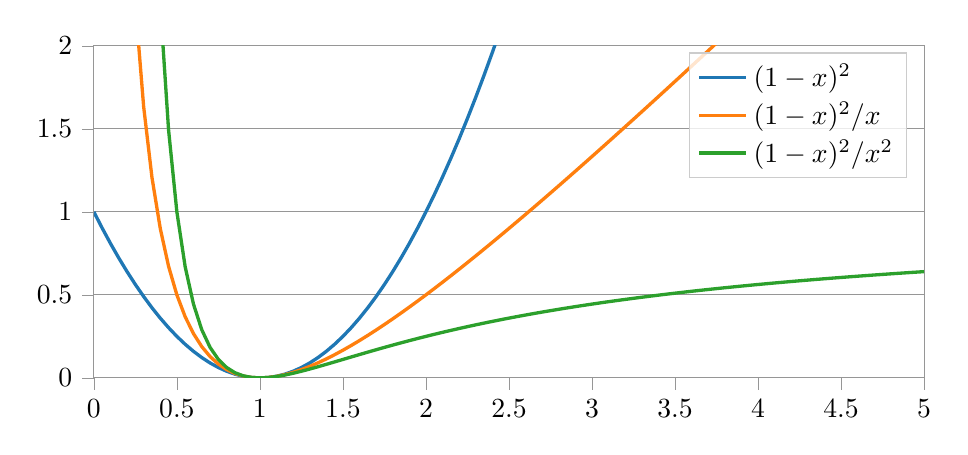
\begin{tikzpicture}

\definecolor{color0}{rgb}{0.12156862745098,0.466666666666667,0.705882352941177}
\definecolor{color1}{rgb}{1,0.498039215686275,0.0549019607843137}
\definecolor{color2}{rgb}{0.172549019607843,0.627450980392157,0.172549019607843}

\begin{axis}[
axis line style={white!58.8235294117647!black},
width=\textwidth,
legend cell align={left},
legend style={
  fill opacity=0.8,
  draw opacity=1,
  text opacity=1,
  % at={(0.91,0.5)},
  % anchor=east,
  draw=white!80!black
},
tick align=outside,
tick pos=left,
x grid style={white!58.8235294117647!black},
xmin=0, xmax=5,
xtick style={color=white!58.8235294117647!black},
y grid style={white!58.8235294117647!black},
ymajorgrids,
ymin=0, ymax=2,
ytick style={color=white!58.8235294117647!black},
unit vector ratio={1 1}
]
\addplot [very thick, color0]
table {%
0 1
0.05 0.9025
0.1 0.81
0.15 0.7225
0.2 0.64
0.25 0.5625
0.3 0.49
0.35 0.4225
0.4 0.36
0.45 0.3025
0.5 0.25
0.55 0.2025
0.6 0.16
0.65 0.1225
0.7 0.09
0.75 0.0625
0.8 0.04
0.85 0.0225
0.9 0.01
0.95 0.00249999999999999
1 0
1.05 0.0025
1.1 0.01
1.15 0.0225
1.2 0.0400000000000001
1.25 0.0625
1.3 0.09
1.35 0.1225
1.4 0.16
1.45 0.2025
1.5 0.25
1.55 0.3025
1.6 0.36
1.65 0.4225
1.7 0.49
1.75 0.5625
1.8 0.64
1.85 0.7225
1.9 0.81
1.95 0.9025
2 1
2.05 1.1025
2.1 1.21
2.15 1.3225
2.2 1.44
2.25 1.5625
2.3 1.69
2.35 1.8225
2.4 1.96
2.45 2.1025
2.5 2.25
2.55 2.4025
2.6 2.56
2.65 2.7225
2.7 2.89
};
\addlegendentry{$(1-x)^2$}
\addplot [very thick, color1]
table {%
0.25 2.25
0.3 1.63333333333333
0.35 1.20714285714286
0.4 0.9
0.45 0.672222222222222
0.5 0.5
0.55 0.368181818181818
0.6 0.266666666666666
0.65 0.188461538461538
0.7 0.128571428571429
0.75 0.0833333333333333
0.8 0.05
0.85 0.0264705882352941
0.9 0.0111111111111111
0.95 0.00263157894736841
1 0
1.05 0.00238095238095239
1.1 0.00909090909090911
1.15 0.0195652173913044
1.2 0.0333333333333334
1.25 0.05
1.3 0.0692307692307692
1.35 0.0907407407407408
1.4 0.114285714285714
1.45 0.139655172413793
1.5 0.166666666666667
1.55 0.195161290322581
1.6 0.225
1.65 0.256060606060606
1.7 0.288235294117647
1.75 0.321428571428571
1.8 0.355555555555556
1.85 0.390540540540541
1.9 0.426315789473684
1.95 0.462820512820513
2 0.5
2.05 0.537804878048781
2.1 0.576190476190476
2.15 0.615116279069767
2.2 0.654545454545455
2.25 0.694444444444444
2.3 0.734782608695652
2.35 0.775531914893617
2.4 0.816666666666667
2.45 0.858163265306123
2.5 0.9
2.55 0.942156862745098
2.6 0.984615384615385
2.65 1.02735849056604
2.7 1.07037037037037
2.75 1.11363636363636
2.8 1.15714285714286
2.85 1.20087719298246
2.9 1.2448275862069
2.95 1.28898305084746
3 1.33333333333333
3.05 1.37786885245902
3.1 1.42258064516129
3.15 1.46746031746032
3.2 1.5125
3.25 1.55769230769231
3.3 1.6030303030303
3.35 1.64850746268657
3.4 1.69411764705882
3.45 1.73985507246377
3.5 1.78571428571429
3.55 1.83169014084507
3.6 1.87777777777778
3.65 1.92397260273973
3.7 1.97027027027027
3.75 2.01666666666667
3.8 2.06315789473684
3.85 2.10974025974026
3.9 2.15641025641026
3.95 2.20316455696203
4 2.25
4.05 2.29691358024691
4.1 2.34390243902439
4.15 2.39096385542169
4.2 2.43809523809524
4.25 2.48529411764706
4.3 2.53255813953488
4.35 2.57988505747127
4.4 2.62727272727273
4.45 2.6747191011236
4.5 2.72222222222222
4.55 2.76978021978022
4.6 2.81739130434783
4.65 2.86505376344086
4.7 2.91276595744681
4.75 2.96052631578947
};
\addlegendentry{$(1-x)^2 / x$}
\addplot [very thick, color2]
table {%
0.4 2.25
0.45 1.49382716049383
0.5 1
0.55 0.669421487603306
0.6 0.444444444444444
0.65 0.289940828402367
0.7 0.183673469387755
0.75 0.111111111111111
0.8 0.0625
0.85 0.0311418685121107
0.9 0.0123456790123457
0.95 0.00277008310249307
1 0
1.05 0.00226757369614513
1.1 0.00826446280991737
1.15 0.0170132325141777
1.2 0.0277777777777778
1.25 0.04
1.3 0.0532544378698225
1.35 0.0672153635116598
1.4 0.0816326530612245
1.45 0.0963139120095125
1.5 0.111111111111111
1.55 0.125910509885536
1.6 0.140625
1.65 0.155188246097337
1.7 0.169550173010381
1.75 0.183673469387755
1.8 0.197530864197531
1.85 0.211102994886779
1.9 0.224376731301939
1.95 0.237343852728468
2 0.25
2.05 0.262343842950625
2.1 0.27437641723356
2.15 0.286100594916171
2.2 0.297520661157025
2.25 0.308641975308642
2.3 0.319470699432892
2.35 0.330013580805794
2.4 0.340277777777778
2.45 0.350270720533111
2.5 0.36
2.55 0.369473279507882
2.6 0.378698224852071
2.65 0.387682449270203
2.7 0.396433470507545
2.75 0.40495867768595
2.8 0.413265306122449
2.85 0.421360418590336
2.9 0.429250891795482
2.95 0.436943407066935
3 0.444444444444444
3.05 0.45176027949476
3.1 0.458896982310094
3.15 0.465860418241371
3.2 0.47265625
3.25 0.479289940828402
3.3 0.485766758494031
3.35 0.492091779906438
3.4 0.498269896193772
3.45 0.50430581810544
3.5 0.510204081632653
3.55 0.515969053759175
3.6 0.521604938271605
3.65 0.527115781572528
3.7 0.532505478451424
3.75 0.537777777777778
3.8 0.542936288088643
3.85 0.547984483049418
3.9 0.552925706771861
3.95 0.557763178977728
4 0.5625
4.05 0.567139155616522
4.1 0.571683521713266
4.15 0.57613586877631
4.2 0.580498866213152
4.25 0.58477508650519
4.3 0.588967009194159
4.35 0.593077024706038
4.4 0.597107438016529
4.45 0.601060472162606
4.5 0.604938271604938
4.55 0.608742905446202
4.6 0.612476370510397
4.65 0.616140594288357
4.7 0.61973743775464
4.75 0.623268698060942
4.8 0.626736111111111
4.85 0.630141354022744
4.9 0.633486047480217
4.95 0.636771757983879
5 0.64
};
\addlegendentry{$(1-x)^2 / x^2$}
\end{axis}

\end{tikzpicture}

  \caption{Different possibilities for the norm-scaling in $p_\text{STRESS}$ with target
  distance 1. The common variant $(1-x)^2$ is a simple quadratic.}
\end{figure}

\begin{figure}
  \centering
  % This file was created with tikzplotlib v0.9.11.
\begin{tikzpicture}
\scriptsize

\begin{axis}[
tick align=outside,
tick pos=left,
ticks=none,
title={XYY},
width=0.4\textwidth,
x grid style={white!69.0196078431373!black},
xlabel={x},
xmin=0.217445, xmax=0.504655,
xtick style={color=black},
y grid style={white!69.0196078431373!black},
ylabel style={rotate=-90.0},
ylabel={y},
ymin=0.246465, ymax=0.555235,
ytick style={color=black}
]
\addplot [draw=black, fill=black, mark=*, only marks]
table [search path={./figures/}]{macadam1974-xyy-000.dat};
\addplot [very thick, black, opacity=0.3]
table {%
0.312 0.5412
0.306483881977648 0.520645893559568
};
\addplot [very thick, black, opacity=0.3]
table {%
0.2952 0.4786
0.300716118022352 0.499154106440432
};
\addplot [very thick, black, opacity=0.3]
table {%
0.312 0.5412
0.325221201942711 0.521597466483784
};
\addplot [very thick, black, opacity=0.3]
table {%
0.3466 0.4899
0.333378798057289 0.509502533516216
};
\addplot [very thick, black, opacity=0.3]
table {%
0.2952 0.4786
0.31467676781135 0.482881857514947
};
\addplot [very thick, black, opacity=0.3]
table {%
0.3466 0.4899
0.32712323218865 0.485618142485053
};
\addplot [very thick, black, opacity=0.3]
table {%
0.2952 0.4786
0.284813822194795 0.461598625869634
};
\addplot [very thick, black, opacity=0.3]
table {%
0.2627 0.4254
0.273086177805205 0.442401374130366
};
\addplot [very thick, black, opacity=0.3]
table {%
0.2952 0.4786
0.298210501332587 0.463789717582217
};
\addplot [very thick, black, opacity=0.3]
table {%
0.3039 0.4358
0.300889498667413 0.450610282417783
};
\addplot [very thick, black, opacity=0.3]
table {%
0.3466 0.4899
0.368320763142334 0.489810058951792
};
\addplot [very thick, black, opacity=0.3]
table {%
0.3949 0.4897
0.373179236857666 0.489789941048208
};
\addplot [very thick, black, opacity=0.3]
table {%
0.3466 0.4899
0.330975945156109 0.470104651825421
};
\addplot [very thick, black, opacity=0.3]
table {%
0.3039 0.4358
0.319524054843891 0.455595348174579
};
\addplot [very thick, black, opacity=0.3]
table {%
0.3466 0.4899
0.34989794171415 0.473331769007482
};
\addplot [very thick, black, opacity=0.3]
table {%
0.355 0.4477
0.35170205828585 0.464268230992518
};
\addplot [very thick, black, opacity=0.3]
table {%
0.3949 0.4897
0.382953859511516 0.47712511527528
};
\addplot [very thick, black, opacity=0.3]
table {%
0.355 0.4477
0.366946140488485 0.460274884724721
};
\addplot [very thick, black, opacity=0.3]
table {%
0.3949 0.4897
0.394191144383037 0.472377340860473
};
\addplot [very thick, black, opacity=0.3]
table {%
0.3933 0.4506
0.394008855616963 0.467922659139527
};
\addplot [very thick, black, opacity=0.3]
table {%
0.2627 0.4254
0.281504881534937 0.430146863300081
};
\addplot [very thick, black, opacity=0.3]
table {%
0.3039 0.4358
0.285095118465063 0.431053136699919
};
\addplot [very thick, black, opacity=0.3]
table {%
0.2627 0.4254
0.253447535492702 0.403208830145844
};
\addplot [very thick, black, opacity=0.3]
table {%
0.2376 0.3652
0.246852464507298 0.387391169854156
};
\addplot [very thick, black, opacity=0.3]
table {%
0.2627 0.4254
0.266558453567003 0.410319877308964
};
\addplot [very thick, black, opacity=0.3]
table {%
0.2747 0.3785
0.270841546432997 0.393580122691036
};
\addplot [very thick, black, opacity=0.3]
table {%
0.3039 0.4358
0.322098464321875 0.440037998540711
};
\addplot [very thick, black, opacity=0.3]
table {%
0.355 0.4477
0.336801535678125 0.443462001459289
};
\addplot [very thick, black, opacity=0.3]
table {%
0.3039 0.4358
0.29530045955553 0.418924874401776
};
\addplot [very thick, black, opacity=0.3]
table {%
0.2747 0.3785
0.28329954044447 0.395375125598224
};
\addplot [very thick, black, opacity=0.3]
table {%
0.3039 0.4358
0.30697396890715 0.424784944749381
};
\addplot [very thick, black, opacity=0.3]
table {%
0.3159 0.3928
0.31282603109285 0.403815055250619
};
\addplot [very thick, black, opacity=0.3]
table {%
0.355 0.4477
0.373061462452644 0.449067578096936
};
\addplot [very thick, black, opacity=0.3]
table {%
0.3933 0.4506
0.375238537547356 0.449232421903064
};
\addplot [very thick, black, opacity=0.3]
table {%
0.355 0.4477
0.346652088179038 0.435978763197677
};
\addplot [very thick, black, opacity=0.3]
table {%
0.3159 0.3928
0.324247911820962 0.404521236802323
};
\addplot [very thick, black, opacity=0.3]
table {%
0.355 0.4477
0.357733313614111 0.430968807574232
};
\addplot [very thick, black, opacity=0.3]
table {%
0.3616 0.4073
0.358866686385889 0.424031192425768
};
\addplot [very thick, black, opacity=0.3]
table {%
0.3933 0.4506
0.418872083108819 0.454846110814711
};
\addplot [very thick, black, opacity=0.3]
table {%
0.4469 0.4595
0.421327916891181 0.455253889185289
};
\addplot [very thick, black, opacity=0.3]
table {%
0.3933 0.4506
0.385579905863891 0.440054887189479
};
\addplot [very thick, black, opacity=0.3]
table {%
0.3616 0.4073
0.369320094136109 0.417845112810521
};
\addplot [very thick, black, opacity=0.3]
table {%
0.3933 0.4506
0.398231269995721 0.432107737516048
};
\addplot [very thick, black, opacity=0.3]
table {%
0.4025 0.4161
0.397568730004279 0.434592262483952
};
\addplot [very thick, black, opacity=0.3]
table {%
0.4469 0.4595
0.432909302067402 0.445824407876695
};
\addplot [very thick, black, opacity=0.3]
table {%
0.4025 0.4161
0.416490697932598 0.429775592123305
};
\addplot [very thick, black, opacity=0.3]
table {%
0.4469 0.4595
0.447303686592254 0.43453871237894
};
\addplot [very thick, black, opacity=0.3]
table {%
0.4475 0.4224
0.447096313407746 0.44736128762106
};
\addplot [very thick, black, opacity=0.3]
table {%
0.2376 0.3652
0.251737092803169 0.370268014401136
};
\addplot [very thick, black, opacity=0.3]
table {%
0.2747 0.3785
0.260562907196832 0.373431985598864
};
\addplot [very thick, black, opacity=0.3]
table {%
0.2376 0.3652
0.233866060277177 0.342217863959528
};
\addplot [very thick, black, opacity=0.3]
table {%
0.2305 0.3215
0.234233939722823 0.344482136040472
};
\addplot [very thick, black, opacity=0.3]
table {%
0.2376 0.3652
0.245924315548048 0.346886505794294
};
\addplot [very thick, black, opacity=0.3]
table {%
0.2531 0.3311
0.244775684451952 0.349413494205706
};
\addplot [very thick, black, opacity=0.3]
table {%
0.2747 0.3785
0.292990453418949 0.384848385531334
};
\addplot [very thick, black, opacity=0.3]
table {%
0.3159 0.3928
0.297609546581051 0.386451614468666
};
\addplot [very thick, black, opacity=0.3]
table {%
0.2747 0.3785
0.26454426474865 0.356213803198426
};
\addplot [very thick, black, opacity=0.3]
table {%
0.2531 0.3311
0.26325573525135 0.353386196801574
};
\addplot [very thick, black, opacity=0.3]
table {%
0.2747 0.3785
0.2793064634866 0.36392610258981
};
\addplot [very thick, black, opacity=0.3]
table {%
0.2863 0.3418
0.281693536513401 0.35637389741019
};
\addplot [very thick, black, opacity=0.3]
table {%
0.3159 0.3928
0.332565152354876 0.398087630397062
};
\addplot [very thick, black, opacity=0.3]
table {%
0.3616 0.4073
0.344934847645123 0.402012369602939
};
\addplot [very thick, black, opacity=0.3]
table {%
0.3159 0.3928
0.30543193698225 0.374763810341039
};
\addplot [very thick, black, opacity=0.3]
table {%
0.2863 0.3418
0.29676806301775 0.359836189658961
};
\addplot [very thick, black, opacity=0.3]
table {%
0.3159 0.3928
0.320148540234156 0.376192069993753
};
\addplot [very thick, black, opacity=0.3]
table {%
0.3247 0.3584
0.320451459765844 0.375007930006247
};
\addplot [very thick, black, opacity=0.3]
table {%
0.3616 0.4073
0.380106766733971 0.411281896021001
};
\addplot [very thick, black, opacity=0.3]
table {%
0.4025 0.4161
0.383993233266029 0.412118103978999
};
\addplot [very thick, black, opacity=0.3]
table {%
0.3616 0.4073
0.351250602074296 0.393584944212279
};
\addplot [very thick, black, opacity=0.3]
table {%
0.3247 0.3584
0.335049397925704 0.372115055787721
};
\addplot [very thick, black, opacity=0.3]
table {%
0.3616 0.4073
0.362148937940552 0.388885627266948
};
\addplot [very thick, black, opacity=0.3]
table {%
0.3627 0.3704
0.362151062059448 0.388814372733052
};
\addplot [very thick, black, opacity=0.3]
table {%
0.4025 0.4161
0.424996736615017 0.419249543126102
};
\addplot [very thick, black, opacity=0.3]
table {%
0.4475 0.4224
0.425003263384983 0.419250456873898
};
\addplot [very thick, black, opacity=0.3]
table {%
0.4025 0.4161
0.392445022547877 0.404554460563769
};
\addplot [very thick, black, opacity=0.3]
table {%
0.3627 0.3704
0.372754977452123 0.381945539436231
};
\addplot [very thick, black, opacity=0.3]
table {%
0.4025 0.4161
0.405374405129093 0.394642231478165
};
\addplot [very thick, black, opacity=0.3]
table {%
0.4068 0.384
0.403925594870907 0.405457768521835
};
\addplot [very thick, black, opacity=0.3]
table {%
0.4475 0.4224
0.463218662545751 0.422268279364142
};
\addplot [very thick, black, opacity=0.3]
table {%
0.4833 0.4221
0.467581337454249 0.422231720635858
};
\addplot [very thick, black, opacity=0.3]
table {%
0.4475 0.4224
0.432161902948288 0.40792867501755
};
\addplot [very thick, black, opacity=0.3]
table {%
0.4068 0.384
0.422138097051712 0.39847132498245
};
\addplot [very thick, black, opacity=0.3]
table {%
0.4475 0.4224
0.446479280080991 0.400709701721064
};
\addplot [very thick, black, opacity=0.3]
table {%
0.4459 0.3884
0.446920719919009 0.410090298278936
};
\addplot [very thick, black, opacity=0.3]
table {%
0.4833 0.4221
0.468234063142036 0.40852454352638
};
\addplot [very thick, black, opacity=0.3]
table {%
0.4459 0.3884
0.460965936857964 0.40197545647362
};
\addplot [very thick, black, opacity=0.3]
table {%
0.4833 0.4221
0.490729427040506 0.399901230047644
};
\addplot [very thick, black, opacity=0.3]
table {%
0.4916 0.3973
0.484170572959494 0.419498769952355
};
\addplot [very thick, black, opacity=0.3]
table {%
0.2305 0.3215
0.24474298652767 0.327550118171046
};
\addplot [very thick, black, opacity=0.3]
table {%
0.2531 0.3311
0.23885701347233 0.325049881828954
};
\addplot [very thick, black, opacity=0.3]
table {%
0.2305 0.3215
0.235873709653899 0.290793087692004
};
\addplot [very thick, black, opacity=0.3]
table {%
0.2368 0.2855
0.231426290346101 0.316206912307996
};
\addplot [very thick, black, opacity=0.3]
table {%
0.2531 0.3311
0.271884950637276 0.337154185898158
};
\addplot [very thick, black, opacity=0.3]
table {%
0.2863 0.3418
0.267515049362724 0.335745814101842
};
\addplot [very thick, black, opacity=0.3]
table {%
0.2531 0.3311
0.242696313799353 0.301995209156471
};
\addplot [very thick, black, opacity=0.3]
table {%
0.2368 0.2855
0.247203686200647 0.314604790843529
};
\addplot [very thick, black, opacity=0.3]
table {%
0.2531 0.3311
0.264698280830012 0.303799431277049
};
\addplot [very thick, black, opacity=0.3]
table {%
0.2661 0.3005
0.254501719169988 0.327800568722951
};
\addplot [very thick, black, opacity=0.3]
table {%
0.2863 0.3418
0.306050987492005 0.350338187301231
};
\addplot [very thick, black, opacity=0.3]
table {%
0.3247 0.3584
0.304949012507995 0.349861812698769
};
\addplot [very thick, black, opacity=0.3]
table {%
0.2863 0.3418
0.274603088287857 0.317885027043985
};
\addplot [very thick, black, opacity=0.3]
table {%
0.2661 0.3005
0.277796911712143 0.324414972956016
};
\addplot [very thick, black, opacity=0.3]
table {%
0.2863 0.3418
0.29677187027001 0.325146817417831
};
\addplot [very thick, black, opacity=0.3]
table {%
0.3007 0.3189
0.29022812972999 0.335553182582169
};
\addplot [very thick, black, opacity=0.3]
table {%
0.3247 0.3584
0.344582999108831 0.364678841823841
};
\addplot [very thick, black, opacity=0.3]
table {%
0.3627 0.3704
0.342817000891169 0.364121158176159
};
\addplot [very thick, black, opacity=0.3]
table {%
0.3247 0.3584
0.31342126342474 0.339837079386551
};
\addplot [very thick, black, opacity=0.3]
table {%
0.3007 0.3189
0.31197873657526 0.33746292061345
};
\addplot [very thick, black, opacity=0.3]
table {%
0.3247 0.3584
0.332277032077758 0.338938991295022
};
\addplot [very thick, black, opacity=0.3]
table {%
0.3342 0.334
0.326622967922242 0.353461008704978
};
\addplot [very thick, black, opacity=0.3]
table {%
0.3627 0.3704
0.376723954442524 0.374724847628534
};
\addplot [very thick, black, opacity=0.3]
table {%
0.4068 0.384
0.392776045557476 0.379675152371466
};
\addplot [very thick, black, opacity=0.3]
table {%
0.3627 0.3704
0.352640999113224 0.357552714656889
};
\addplot [very thick, black, opacity=0.3]
table {%
0.3342 0.334
0.344259000886776 0.346847285343111
};
\addplot [very thick, black, opacity=0.3]
table {%
0.3627 0.3704
0.371571542117589 0.350498973087571
};
\addplot [very thick, black, opacity=0.3]
table {%
0.3738 0.3455
0.364928457882411 0.365401026912429
};
\addplot [very thick, black, opacity=0.3]
table {%
0.4068 0.384
0.419738249924628 0.385455966743436
};
\addplot [very thick, black, opacity=0.3]
table {%
0.4459 0.3884
0.432961750075372 0.386944033256564
};
\addplot [very thick, black, opacity=0.3]
table {%
0.4068 0.384
0.396979136475784 0.372542325888415
};
\addplot [very thick, black, opacity=0.3]
table {%
0.3738 0.3455
0.383620863524216 0.356957674111585
};
\addplot [very thick, black, opacity=0.3]
table {%
0.4068 0.384
0.408412392864676 0.364211542115345
};
\addplot [very thick, black, opacity=0.3]
table {%
0.409 0.357
0.407387607135324 0.376788457884655
};
\addplot [very thick, black, opacity=0.3]
table {%
0.4459 0.3884
0.461460304138491 0.391430343694367
};
\addplot [very thick, black, opacity=0.3]
table {%
0.4916 0.3973
0.476039695861509 0.394269656305633
};
\addplot [very thick, black, opacity=0.3]
table {%
0.4459 0.3884
0.432744684687809 0.377205504043284
};
\addplot [very thick, black, opacity=0.3]
table {%
0.409 0.357
0.422155315312191 0.368194495956716
};
\addplot [very thick, black, opacity=0.3]
table {%
0.4459 0.3884
0.456449248858165 0.368201050635916
};
\addplot [very thick, black, opacity=0.3]
table {%
0.4588 0.3637
0.448250751141835 0.383898949364084
};
\addplot [very thick, black, opacity=0.3]
table {%
0.4916 0.3973
0.473555881049395 0.378815780587185
};
\addplot [very thick, black, opacity=0.3]
table {%
0.4588 0.3637
0.476844118950605 0.382184219412815
};
\addplot [very thick, black, opacity=0.3]
table {%
0.4916 0.3973
0.488192274989554 0.373808448864159
};
\addplot [very thick, black, opacity=0.3]
table {%
0.4869 0.3649
0.490307725010446 0.388391551135841
};
\addplot [very thick, black, opacity=0.3]
table {%
0.2368 0.2855
0.255106405753469 0.294871880078568
};
\addplot [very thick, black, opacity=0.3]
table {%
0.2661 0.3005
0.247793594246531 0.291128119921432
};
\addplot [very thick, black, opacity=0.3]
table {%
0.2368 0.2855
0.252433539013253 0.261066124456107
};
\addplot [very thick, black, opacity=0.3]
table {%
0.2519 0.2619
0.236266460986747 0.286333875543893
};
\addplot [very thick, black, opacity=0.3]
table {%
0.2661 0.3005
0.28334198365955 0.309669147379645
};
\addplot [very thick, black, opacity=0.3]
table {%
0.3007 0.3189
0.28345801634045 0.309730852620355
};
\addplot [very thick, black, opacity=0.3]
table {%
0.2661 0.3005
0.256742257798343 0.275062757113806
};
\addplot [very thick, black, opacity=0.3]
table {%
0.2519 0.2619
0.261257742201657 0.287337242886194
};
\addplot [very thick, black, opacity=0.3]
table {%
0.2661 0.3005
0.279810606797119 0.28124466251287
};
\addplot [very thick, black, opacity=0.3]
table {%
0.2797 0.2814
0.265989393202881 0.30065533748713
};
\addplot [very thick, black, opacity=0.3]
table {%
0.3007 0.3189
0.314964352326181 0.325329603585831
};
\addplot [very thick, black, opacity=0.3]
table {%
0.3342 0.334
0.319935647673819 0.327570396414169
};
\addplot [very thick, black, opacity=0.3]
table {%
0.3007 0.3189
0.288429101181314 0.296987680680918
};
\addplot [very thick, black, opacity=0.3]
table {%
0.2797 0.2814
0.291970898818686 0.303312319319082
};
\addplot [very thick, black, opacity=0.3]
table {%
0.3007 0.3189
0.305767218695405 0.298542226644776
};
\addplot [very thick, black, opacity=0.3]
table {%
0.3064 0.296
0.301332781304595 0.316357773355224
};
\addplot [very thick, black, opacity=0.3]
table {%
0.3342 0.334
0.351729084436959 0.339090516945076
};
\addplot [very thick, black, opacity=0.3]
table {%
0.3738 0.3455
0.356270915563041 0.340409483054924
};
\addplot [very thick, black, opacity=0.3]
table {%
0.3342 0.334
0.319759014700712 0.314260523691621
};
\addplot [very thick, black, opacity=0.3]
table {%
0.3064 0.296
0.320840985299288 0.315739476308379
};
\addplot [very thick, black, opacity=0.3]
table {%
0.3342 0.334
0.338845352270254 0.318975188750896
};
\addplot [very thick, black, opacity=0.3]
table {%
0.3406 0.3133
0.335954647729746 0.328324811249104
};
\addplot [very thick, black, opacity=0.3]
table {%
0.3738 0.3455
0.385790746690292 0.349417431447112
};
\addplot [very thick, black, opacity=0.3]
table {%
0.409 0.357
0.397009253309708 0.353082568552888
};
\addplot [very thick, black, opacity=0.3]
table {%
0.3738 0.3455
0.360116172107796 0.332228335598525
};
\addplot [very thick, black, opacity=0.3]
table {%
0.3406 0.3133
0.354283827892204 0.326571664401475
};
\addplot [very thick, black, opacity=0.3]
table {%
0.3738 0.3455
0.377182026412342 0.332869166664109
};
\addplot [very thick, black, opacity=0.3]
table {%
0.3787 0.3272
0.375317973587658 0.339830833335891
};
\addplot [very thick, black, opacity=0.3]
table {%
0.409 0.357
0.427575678129809 0.359499137419071
};
\addplot [very thick, black, opacity=0.3]
table {%
0.4588 0.3637
0.440224321870191 0.361200862580929
};
\addplot [very thick, black, opacity=0.3]
table {%
0.409 0.357
0.392702993045004 0.340971920552512
};
\addplot [very thick, black, opacity=0.3]
table {%
0.3787 0.3272
0.394997006954996 0.343228079447488
};
\addplot [very thick, black, opacity=0.3]
table {%
0.409 0.357
0.416955829482432 0.339920512854227
};
\addplot [very thick, black, opacity=0.3]
table {%
0.4199 0.3336
0.411944170517567 0.350679487145773
};
\addplot [very thick, black, opacity=0.3]
table {%
0.4588 0.3637
0.469820821766254 0.364170640075427
};
\addplot [very thick, black, opacity=0.3]
table {%
0.4869 0.3649
0.475879178233746 0.364429359924573
};
\addplot [very thick, black, opacity=0.3]
table {%
0.4588 0.3637
0.440617675909396 0.349630900896474
};
\addplot [very thick, black, opacity=0.3]
table {%
0.4199 0.3336
0.438082324090604 0.347669099103526
};
\addplot [very thick, black, opacity=0.3]
table {%
0.4588 0.3637
0.455878119874647 0.341210377216982
};
\addplot [very thick, black, opacity=0.3]
table {%
0.4555 0.3383
0.458421880125353 0.360789622783018
};
\addplot [very thick, black, opacity=0.3]
table {%
0.4869 0.3649
0.468833795801933 0.349595508545586
};
\addplot [very thick, black, opacity=0.3]
table {%
0.4555 0.3383
0.473566204198067 0.353604491454413
};
\addplot [very thick, black, opacity=0.3]
table {%
0.2519 0.2619
0.272393825526954 0.276275165387612
};
\addplot [very thick, black, opacity=0.3]
table {%
0.2797 0.2814
0.259206174473046 0.267024834612388
};
\addplot [very thick, black, opacity=0.3]
table {%
0.2797 0.2814
0.292670600149106 0.288492537909249
};
\addplot [very thick, black, opacity=0.3]
table {%
0.3064 0.296
0.293429399850894 0.288907462090751
};
\addplot [very thick, black, opacity=0.3]
table {%
0.2797 0.2814
0.29159573663875 0.263767312358164
};
\addplot [very thick, black, opacity=0.3]
table {%
0.2938 0.2605
0.28190426336125 0.278132687641836
};
\addplot [very thick, black, opacity=0.3]
table {%
0.3064 0.296
0.321975305806296 0.303878736562834
};
\addplot [very thick, black, opacity=0.3]
table {%
0.3406 0.3133
0.325024694193704 0.305421263437166
};
\addplot [very thick, black, opacity=0.3]
table {%
0.3064 0.296
0.299872790799606 0.277609847094128
};
\addplot [very thick, black, opacity=0.3]
table {%
0.2938 0.2605
0.300327209200394 0.278890152905872
};
\addplot [very thick, black, opacity=0.3]
table {%
0.3064 0.296
0.319226968486779 0.278472465421793
};
\addplot [very thick, black, opacity=0.3]
table {%
0.3225 0.274
0.309673031513221 0.291527534578207
};
\addplot [very thick, black, opacity=0.3]
table {%
0.3406 0.3133
0.356683788289984 0.319167838772461
};
\addplot [very thick, black, opacity=0.3]
table {%
0.3787 0.3272
0.362616211710016 0.321332161227539
};
\addplot [very thick, black, opacity=0.3]
table {%
0.3406 0.3133
0.329620629685768 0.289460814732083
};
\addplot [very thick, black, opacity=0.3]
table {%
0.3225 0.274
0.333479370314232 0.297839185267918
};
\addplot [very thick, black, opacity=0.3]
table {%
0.3406 0.3133
0.351885244979383 0.298679214632623
};
\addplot [very thick, black, opacity=0.3]
table {%
0.3609 0.287
0.349614755020617 0.301620785367377
};
\addplot [very thick, black, opacity=0.3]
table {%
0.3787 0.3272
0.392240150630713 0.329303324369819
};
\addplot [very thick, black, opacity=0.3]
table {%
0.4199 0.3336
0.406359849369287 0.331496675630181
};
\addplot [very thick, black, opacity=0.3]
table {%
0.3787 0.3272
0.369651751257931 0.306765191043192
};
\addplot [very thick, black, opacity=0.3]
table {%
0.3609 0.287
0.369948248742069 0.307434808956808
};
\addplot [very thick, black, opacity=0.3]
table {%
0.3787 0.3272
0.384091988555093 0.30453999746467
};
\addplot [very thick, black, opacity=0.3]
table {%
0.3866 0.294
0.381208011444907 0.31666000253533
};
\addplot [very thick, black, opacity=0.3]
table {%
0.4199 0.3336
0.433181233382894 0.335353421261225
};
\addplot [very thick, black, opacity=0.3]
table {%
0.4555 0.3383
0.442218766617106 0.336546578738775
};
\addplot [very thick, black, opacity=0.3]
table {%
0.4199 0.3336
0.402494266670495 0.312901290094643
};
\addplot [very thick, black, opacity=0.3]
table {%
0.3866 0.294
0.404005733329505 0.314698709905357
};
\addplot [very thick, black, opacity=0.3]
table {%
0.2938 0.2605
0.311529325918694 0.268839578393811
};
\addplot [very thick, black, opacity=0.3]
table {%
0.3225 0.274
0.304770674081306 0.265660421606189
};
\addplot [very thick, black, opacity=0.3]
table {%
0.3225 0.274
0.340811343991049 0.280199152913637
};
\addplot [very thick, black, opacity=0.3]
table {%
0.3609 0.287
0.342588656008951 0.280800847086364
};
\addplot [very thick, black, opacity=0.3]
table {%
0.3609 0.287
0.371863428259129 0.28998614777486
};
\addplot [very thick, black, opacity=0.3]
table {%
0.3866 0.294
0.375636571740871 0.29101385222514
};
\end{axis}

\end{tikzpicture}

  \hfill
  % This file was created with tikzplotlib v0.9.11.
\begin{tikzpicture}
\scriptsize

\begin{axis}[
tick align=outside,
tick pos=left,
ticks=none,
title={CIELAB},
width=0.4\textwidth,
x grid style={white!69.0196078431373!black},
xlabel={a*},
xmin=-56.2677416958569, xmax=44.931737286182,
xtick style={color=black},
y grid style={white!69.0196078431373!black},
ylabel style={rotate=-90.0},
ylabel={b*},
ymin=-30.3404617516908, ymax=59.2639321832299,
ytick style={color=black}
]
\addplot [draw=black, fill=black, mark=*, only marks]
table [search path={./figures/}]{macadam1974-cielab-000.dat};
\addplot [very thick, black, opacity=0.3]
table {%
-51.6677653784915 49.9167019659692
-49.0832185938884 43.255582106
};
\addplot [very thick, black, opacity=0.3]
table {%
-44.9095383449791 32.4988085932153
-47.4940851295822 39.1599284531845
};
\addplot [very thick, black, opacity=0.3]
table {%
-51.6677653784915 49.9167019659692
-44.0034588706876 47.4350388194757
};
\addplot [very thick, black, opacity=0.3]
table {%
-31.1176714253977 43.2626869199314
-38.7819779332017 45.744350066425
};
\addplot [very thick, black, opacity=0.3]
table {%
-44.9095383449791 32.4988085932153
-39.6073905731596 36.6368758917842
};
\addplot [very thick, black, opacity=0.3]
table {%
-31.1176714253977 43.2626869199314
-36.4198191972172 39.1246196213625
};
\addplot [very thick, black, opacity=0.3]
table {%
-44.9095383449791 32.4988085932153
-44.7823352314432 25.8212664042187
};
\addplot [very thick, black, opacity=0.3]
table {%
-44.6039570652229 16.4572838929231
-44.7311601787587 23.1348260819196
};
\addplot [very thick, black, opacity=0.3]
table {%
-44.9095383449791 32.4988085932153
-40.3010495806582 29.3485494690317
};
\addplot [very thick, black, opacity=0.3]
table {%
-32.0211640116885 23.6886061785574
-36.6296527760093 26.8388653027411
};
\addplot [very thick, black, opacity=0.3]
table {%
-31.1176714253977 43.2626869199314
-24.389184485333 47.3841912130079
};
\addplot [very thick, black, opacity=0.3]
table {%
-17.260899785859 51.7505898183488
-23.9893867259238 47.6290855252723
};
\addplot [very thick, black, opacity=0.3]
table {%
-31.1176714253977 43.2626869199314
-31.5143846374032 34.6679330051863
};
\addplot [very thick, black, opacity=0.3]
table {%
-32.0211640116885 23.6886061785574
-31.624450799683 32.2833600933025
};
\addplot [very thick, black, opacity=0.3]
table {%
-31.1176714253977 43.2626869199314
-26.2013221050745 39.3949142736609
};
\addplot [very thick, black, opacity=0.3]
table {%
-18.9794323248966 33.713335133081
-23.8957816452198 37.5811077793515
};
\addplot [very thick, black, opacity=0.3]
table {%
-17.260899785859 51.7505898183488
-17.8114824228506 45.971822746376
};
\addplot [very thick, black, opacity=0.3]
table {%
-18.9794323248966 33.713335133081
-18.428849687905 39.4921022050538
};
\addplot [very thick, black, opacity=0.3]
table {%
-17.260899785859 51.7505898183488
-13.4583369592874 46.4576065537788
};
\addplot [very thick, black, opacity=0.3]
table {%
-8.82754365439349 40.0117665815343
-12.6301064809651 45.3047498461043
};
\addplot [very thick, black, opacity=0.3]
table {%
-44.6039570652229 16.4572838929231
-38.5567631838237 19.9326019478306
};
\addplot [very thick, black, opacity=0.3]
table {%
-32.0211640116885 23.6886061785574
-38.0683578930876 20.2132881236499
};
\addplot [very thick, black, opacity=0.3]
table {%
-44.6039570652229 16.4572838929231
-42.2189012890152 8.77178727428111
};
\addplot [very thick, black, opacity=0.3]
table {%
-39.5120064102235 0.0492107855033515
-41.8970621864312 7.7347074041453
};
\addplot [very thick, black, opacity=0.3]
table {%
-44.6039570652229 16.4572838929231
-39.8946516363932 13.8366392502035
};
\addplot [very thick, black, opacity=0.3]
table {%
-28.2143437519846 7.33675582892429
-32.9236491808142 9.95740047164382
};
\addplot [very thick, black, opacity=0.3]
table {%
-32.0211640116885 23.6886061785574
-27.0251194546154 27.5288931689809
};
\addplot [very thick, black, opacity=0.3]
table {%
-18.9794323248966 33.713335133081
-23.9754768819697 29.8730481426575
};
\addplot [very thick, black, opacity=0.3]
table {%
-32.0211640116885 23.6886061785574
-30.5811813532006 17.5032915770502
};
\addplot [very thick, black, opacity=0.3]
table {%
-28.2143437519846 7.33675582892429
-29.6543264104724 13.5220704304315
};
\addplot [very thick, black, opacity=0.3]
table {%
-32.0211640116885 23.6886061785574
-28.6743771985609 21.8172352930458
};
\addplot [very thick, black, opacity=0.3]
table {%
-17.6259470087366 15.6394559057403
-20.9727338218641 17.510826791252
};
\addplot [very thick, black, opacity=0.3]
table {%
-18.9794323248966 33.713335133081
-13.1881957941259 37.3063322072924
};
\addplot [very thick, black, opacity=0.3]
table {%
-8.82754365439349 40.0117665815343
-14.6187801851642 36.4187695073228
};
\addplot [very thick, black, opacity=0.3]
table {%
-18.9794323248966 33.713335133081
-18.6192215649867 28.9032306618551
};
\addplot [very thick, black, opacity=0.3]
table {%
-17.6259470087366 15.6394559057403
-17.9861577686465 20.4495603769662
};
\addplot [very thick, black, opacity=0.3]
table {%
-18.9794323248966 33.713335133081
-14.0167021579245 30.2995840632301
};
\addplot [very thick, black, opacity=0.3]
table {%
-7.41274453922205 25.7568693421817
-12.3754747061941 29.1706204120325
};
\addplot [very thick, black, opacity=0.3]
table {%
-8.82754365439349 40.0117665815343
-3.40877208375631 47.2858757109992
};
\addplot [very thick, black, opacity=0.3]
table {%
2.48007149831833 55.1910051861881
-2.93870007231885 47.9168960567232
};
\addplot [very thick, black, opacity=0.3]
table {%
-8.82754365439349 40.0117665815343
-8.32025451304632 34.900543014175
};
\addplot [very thick, black, opacity=0.3]
table {%
-7.41274453922205 25.7568693421817
-7.92003368056923 30.868092909541
};
\addplot [very thick, black, opacity=0.3]
table {%
-8.82754365439349 40.0117665815343
-2.07801910412085 36.3717725014735
};
\addplot [very thick, black, opacity=0.3]
table {%
1.91082608190869 34.2206027775498
-4.83869846836395 37.8605968576106
};
\addplot [very thick, black, opacity=0.3]
table {%
2.48007149831833 55.1910051861881
2.30116960642427 48.6004476576838
};
\addplot [very thick, black, opacity=0.3]
table {%
1.91082608190869 34.2206027775498
2.08972797380275 40.8111603060541
};
\addplot [very thick, black, opacity=0.3]
table {%
2.48007149831833 55.1910051861881
8.09021908562753 48.9000944180306
};
\addplot [very thick, black, opacity=0.3]
table {%
11.9481727889926 44.5739974450287
6.3380252016834 50.8649082131862
};
\addplot [very thick, black, opacity=0.3]
table {%
-39.5120064102235 0.0492107855033515
-35.0958206707269 2.89786660664573
};
\addplot [very thick, black, opacity=0.3]
table {%
-28.2143437519846 7.33675582892429
-32.6305294914813 4.48810000778191
};
\addplot [very thick, black, opacity=0.3]
table {%
-39.5120064102235 0.0492107855033515
-34.5315220122053 -6.00883057341623
};
\addplot [very thick, black, opacity=0.3]
table {%
-30.0345612811173 -11.4787350889707
-35.0150456791355 -5.42069373005113
};
\addplot [very thick, black, opacity=0.3]
table {%
-39.5120064102235 0.0492107855033515
-33.2687887069783 -2.4710958738567
};
\addplot [very thick, black, opacity=0.3]
table {%
-23.3200550127778 -6.48727166229033
-29.563272716023 -3.96696500293027
};
\addplot [very thick, black, opacity=0.3]
table {%
-28.2143437519846 7.33675582892429
-23.0557706816453 11.3817577367607
};
\addplot [very thick, black, opacity=0.3]
table {%
-17.6259470087366 15.6394559057403
-22.7845200790759 11.5944539979039
};
\addplot [very thick, black, opacity=0.3]
table {%
-28.2143437519846 7.33675582892429
-25.4068519285206 -0.593067321480307
};
\addplot [very thick, black, opacity=0.3]
table {%
-23.3200550127778 -6.48727166229033
-26.1275468362418 1.44255148811427
};
\addplot [very thick, black, opacity=0.3]
table {%
-28.2143437519846 7.33675582892429
-23.6335966070121 5.05353632304308
};
\addplot [very thick, black, opacity=0.3]
table {%
-13.5567773892282 0.0308643730023575
-18.1375245342008 2.31408387888357
};
\addplot [very thick, black, opacity=0.3]
table {%
-17.6259470087366 15.6394559057403
-13.3674092148858 19.8580531208357
};
\addplot [very thick, black, opacity=0.3]
table {%
-7.41274453922205 25.7568693421817
-11.6712823330728 21.5382721270863
};
\addplot [very thick, black, opacity=0.3]
table {%
-17.6259470087366 15.6394559057403
-15.8498288971516 8.82659119134725
};
\addplot [very thick, black, opacity=0.3]
table {%
-13.5567773892282 0.0308643730023575
-15.3328955008133 6.84372908739545
};
\addplot [very thick, black, opacity=0.3]
table {%
-17.6259470087366 15.6394559057403
-12.2939900114012 12.7206492672074
};
\addplot [very thick, black, opacity=0.3]
table {%
-5.23797685311874 8.85806409289664
-10.5699338504542 11.7768707314296
};
\addplot [very thick, black, opacity=0.3]
table {%
-7.41274453922205 25.7568693421817
-2.56941650292487 30.1535365746215
};
\addplot [very thick, black, opacity=0.3]
table {%
1.91082608190869 34.2206027775498
-2.93250195438849 29.82393554511
};
\addplot [very thick, black, opacity=0.3]
table {%
-7.41274453922205 25.7568693421817
-6.67853324226624 20.0517571141661
};
\addplot [very thick, black, opacity=0.3]
table {%
-5.23797685311874 8.85806409289664
-5.97218815007454 14.5631763209122
};
\addplot [very thick, black, opacity=0.3]
table {%
-7.41274453922205 25.7568693421817
-2.64603259378722 21.8444709608267
};
\addplot [very thick, black, opacity=0.3]
table {%
3.29337498668722 16.9695532250673
-1.47333695874761 20.8819516064224
};
\addplot [very thick, black, opacity=0.3]
table {%
1.91082608190869 34.2206027775498
7.21008706443326 39.6867226595428
};
\addplot [very thick, black, opacity=0.3]
table {%
11.9481727889926 44.5739974450287
6.64891180646803 39.1078775630356
};
\addplot [very thick, black, opacity=0.3]
table {%
1.91082608190869 34.2206027775498
2.32730505512229 29.0238973448217
};
\addplot [very thick, black, opacity=0.3]
table {%
3.29337498668722 16.9695532250673
2.87689601347362 22.1662586577954
};
\addplot [very thick, black, opacity=0.3]
table {%
1.91082608190869 34.2206027775498
7.94213093752786 29.9571440679758
};
\addplot [very thick, black, opacity=0.3]
table {%
12.0744166253179 27.0360797497558
6.04311176969869 31.2995384593298
};
\addplot [very thick, black, opacity=0.3]
table {%
11.9481727889926 44.5739974450287
15.8694381974131 48.2408078814306
};
\addplot [very thick, black, opacity=0.3]
table {%
20.5744527434157 52.6405091624654
16.6531873349952 48.9736987260635
};
\addplot [very thick, black, opacity=0.3]
table {%
11.9481727889926 44.5739974450287
11.9995842233182 37.4318705100205
};
\addplot [very thick, black, opacity=0.3]
table {%
12.0744166253179 27.0360797497558
12.0230051909923 34.178206684764
};
\addplot [very thick, black, opacity=0.3]
table {%
11.9481727889926 44.5739974450287
17.2602231818668 39.2533231797582
};
\addplot [very thick, black, opacity=0.3]
table {%
21.3122181350326 35.1947499969368
16.0001677421584 40.5154242622073
};
\addplot [very thick, black, opacity=0.3]
table {%
20.5744527434157 52.6405091624654
20.8757676751677 45.515388098164
};
\addplot [very thick, black, opacity=0.3]
table {%
21.3122181350326 35.1947499969368
21.0109032032807 42.3198710612383
};
\addplot [very thick, black, opacity=0.3]
table {%
20.5744527434157 52.6405091624654
27.1138122322289 48.3006471399469
};
\addplot [very thick, black, opacity=0.3]
table {%
29.4714872979231 46.7359702787728
22.9321278091099 51.0758323012913
};
\addplot [very thick, black, opacity=0.3]
table {%
-30.0345612811173 -11.4787350889707
-25.7985190759711 -8.32972473796976
};
\addplot [very thick, black, opacity=0.3]
table {%
-23.3200550127778 -6.48727166229033
-27.556097217924 -9.63628201329128
};
\addplot [very thick, black, opacity=0.3]
table {%
-30.0345612811173 -11.4787350889707
-20.9948728328398 -16.8389814400889
};
\addplot [very thick, black, opacity=0.3]
table {%
-14.7895943495352 -20.5185132666691
-23.8292827978126 -15.1582669155509
};
\addplot [very thick, black, opacity=0.3]
table {%
-23.3200550127778 -6.48727166229033
-17.5616404961053 -2.64285274740245
};
\addplot [very thick, black, opacity=0.3]
table {%
-13.5567773892282 0.0308643730023575
-19.3151919059007 -3.81355454188552
};
\addplot [very thick, black, opacity=0.3]
table {%
-23.3200550127778 -6.48727166229033
-17.9459695748227 -15.3267815269145
};
\addplot [very thick, black, opacity=0.3]
table {%
-14.7895943495352 -20.5185132666691
-20.1636797874903 -11.6790034020449
};
\addplot [very thick, black, opacity=0.3]
table {%
-23.3200550127778 -6.48727166229033
-14.1560164490487 -10.4053252408768
};
\addplot [very thick, black, opacity=0.3]
table {%
-7.78953888485512 -13.1272911110453
-16.9535774485842 -9.20923753245888
};
\addplot [very thick, black, opacity=0.3]
table {%
-13.5567773892282 0.0308643730023575
-8.5919362558887 5.29912919931957
};
\addplot [very thick, black, opacity=0.3]
table {%
-5.23797685311874 8.85806409289664
-10.2028179864583 3.58979926657943
};
\addplot [very thick, black, opacity=0.3]
table {%
-13.5567773892282 0.0308643730023575
-9.82318453348082 -8.48745774473261
};
\addplot [very thick, black, opacity=0.3]
table {%
-7.78953888485512 -13.1272911110453
-11.5231317406026 -4.60896899331038
};
\addplot [very thick, black, opacity=0.3]
table {%
-13.5567773892282 0.0308643730023575
-6.01235865998024 -2.45722619542911
};
\addplot [very thick, black, opacity=0.3]
table {%
-0.890139810068928 -4.1464940989322
-8.43455853931694 -1.65840353050073
};
\addplot [very thick, black, opacity=0.3]
table {%
-5.23797685311874 8.85806409289664
-0.179473047198746 13.667618242957
};
\addplot [very thick, black, opacity=0.3]
table {%
3.29337498668722 16.9695532250673
-1.76512881923277 12.1599990750069
};
\addplot [very thick, black, opacity=0.3]
table {%
-5.23797685311874 8.85806409289664
-2.83638999256339 1.67481969537523
};
\addplot [very thick, black, opacity=0.3]
table {%
-0.890139810068928 -4.1464940989322
-3.29172667062428 3.0367502985892
};
\addplot [very thick, black, opacity=0.3]
table {%
-5.23797685311874 8.85806409289664
1.4740523782236 5.82420473874617
};
\addplot [very thick, black, opacity=0.3]
table {%
5.64904789880169 3.93709299100591
-1.06298133254065 6.97095234515638
};
\addplot [very thick, black, opacity=0.3]
table {%
3.29337498668722 16.9695532250673
6.54197839307622 20.6937301171049
};
\addplot [very thick, black, opacity=0.3]
table {%
12.0744166253179 27.0360797497558
8.82581321892887 23.3119028577182
};
\addplot [very thick, black, opacity=0.3]
table {%
3.29337498668722 16.9695532250673
4.27771110687678 11.5238390610385
};
\addplot [very thick, black, opacity=0.3]
table {%
5.64904789880169 3.93709299100591
4.66471177861213 9.3828071550347
};
\addplot [very thick, black, opacity=0.3]
table {%
3.29337498668722 16.9695532250673
10.0257807146292 14.1668201884976
};
\addplot [very thick, black, opacity=0.3]
table {%
14.5634628467433 12.2777611901155
7.83105711880141 15.0804942266852
};
\addplot [very thick, black, opacity=0.3]
table {%
12.0744166253179 27.0360797497558
15.3405377697994 29.9206627727995
};
\addplot [very thick, black, opacity=0.3]
table {%
21.3122181350326 35.1947499969368
18.046096990551 32.3101669738931
};
\addplot [very thick, black, opacity=0.3]
table {%
12.0744166253179 27.0360797497558
12.9189838934132 22.0283813469282
};
\addplot [very thick, black, opacity=0.3]
table {%
14.5634628467433 12.2777611901155
13.718895578648 17.2854595929431
};
\addplot [very thick, black, opacity=0.3]
table {%
12.0744166253179 27.0360797497558
17.4855402715666 23.1217648717938
};
\addplot [very thick, black, opacity=0.3]
table {%
21.1346470473004 20.4820630506333
15.7235234010517 24.3963779285953
};
\addplot [very thick, black, opacity=0.3]
table {%
21.3122181350326 35.1947499969368
24.5843339099106 39.8231313129123
};
\addplot [very thick, black, opacity=0.3]
table {%
29.4714872979231 46.7359702787728
26.1993715230451 42.1075889627973
};
\addplot [very thick, black, opacity=0.3]
table {%
21.3122181350326 35.1947499969368
21.2423573682412 29.406422602213
};
\addplot [very thick, black, opacity=0.3]
table {%
21.1346470473004 20.4820630506333
21.2045078140919 26.2703904453571
};
\addplot [very thick, black, opacity=0.3]
table {%
21.3122181350326 35.1947499969368
28.4575509208891 32.2001487779863
};
\addplot [very thick, black, opacity=0.3]
table {%
32.2611196802441 30.6060772372356
25.1157868943877 33.6006784561861
};
\addplot [very thick, black, opacity=0.3]
table {%
29.4714872979231 46.7359702787728
30.9992418881086 37.9023625641583
};
\addplot [very thick, black, opacity=0.3]
table {%
32.2611196802441 30.6060772372356
30.7333650900586 39.4396849518501
};
\addplot [very thick, black, opacity=0.3]
table {%
29.4714872979231 46.7359702787728
35.882327710946 40.2408149656197
};
\addplot [very thick, black, opacity=0.3]
table {%
39.2957129980358 36.7825370870683
32.8848725850129 43.2776924002214
};
\addplot [very thick, black, opacity=0.3]
table {%
-14.7895943495352 -20.5185132666691
-10.0440563682726 -15.5077921881805
};
\addplot [very thick, black, opacity=0.3]
table {%
-7.78953888485512 -13.1272911110453
-12.5350768661177 -18.138012189534
};
\addplot [very thick, black, opacity=0.3]
table {%
-14.7895943495352 -20.5185132666691
-4.93324561270141 -24.0321685192403
};
\addplot [very thick, black, opacity=0.3]
table {%
1.33730388261651 -26.2675347546489
-8.51904485421727 -22.7538795020778
};
\addplot [very thick, black, opacity=0.3]
table {%
-7.78953888485512 -13.1272911110453
-3.78607635263574 -7.9160714152812
};
\addplot [very thick, black, opacity=0.3]
table {%
-0.890139810068928 -4.1464940989322
-4.89360234228831 -9.35771379469634
};
\addplot [very thick, black, opacity=0.3]
table {%
-7.78953888485512 -13.1272911110453
-2.50100087325337 -20.74138941003
};
\addplot [very thick, black, opacity=0.3]
table {%
1.33730388261651 -26.2675347546489
-3.95123412898524 -18.6534364556643
};
\addplot [very thick, black, opacity=0.3]
table {%
-7.78953888485512 -13.1272911110453
0.279891619455533 -15.6683298576844
};
\addplot [very thick, black, opacity=0.3]
table {%
5.06951261195771 -17.1765667174184
-2.99991789235295 -14.6355279707794
};
\addplot [very thick, black, opacity=0.3]
table {%
-0.890139810068928 -4.1464940989322
2.92759233305186 0.572894858676254
};
\addplot [very thick, black, opacity=0.3]
table {%
5.64904789880169 3.93709299100591
1.83131575568091 -0.782295966602544
};
\addplot [very thick, black, opacity=0.3]
table {%
-0.890139810068928 -4.1464940989322
2.6253662445955 -11.8327308018821
};
\addplot [very thick, black, opacity=0.3]
table {%
5.06951261195771 -17.1765667174184
1.55400655729328 -9.4903300144685
};
\addplot [very thick, black, opacity=0.3]
table {%
-0.890139810068928 -4.1464940989322
5.97358638887925 -7.73581929058429
};
\addplot [very thick, black, opacity=0.3]
table {%
9.56404182978014 -9.61341635520857
2.70031563083196 -6.02409116355648
};
\addplot [very thick, black, opacity=0.3]
table {%
5.64904789880169 3.93709299100591
10.1890787141006 8.18491978225087
};
\addplot [very thick, black, opacity=0.3]
table {%
14.5634628467433 12.2777611901155
10.0234320314444 8.02993439887053
};
\addplot [very thick, black, opacity=0.3]
table {%
5.64904789880169 3.93709299100591
7.98592493490813 -4.15126542716417
};
\addplot [very thick, black, opacity=0.3]
table {%
9.56404182978014 -9.61341635520857
7.2271647936737 -1.52505793703849
};
\addplot [very thick, black, opacity=0.3]
table {%
5.64904789880169 3.93709299100591
11.0765433524516 1.33248073362409
};
\addplot [very thick, black, opacity=0.3]
table {%
15.1890282300441 -0.641068320806069
9.7615327763942 1.96354393657575
};
\addplot [very thick, black, opacity=0.3]
table {%
14.5634628467433 12.2777611901155
17.2094930621511 15.5814017451034
};
\addplot [very thick, black, opacity=0.3]
table {%
21.1346470473004 20.4820630506333
18.4886168318927 17.1784224956454
};
\addplot [very thick, black, opacity=0.3]
table {%
14.5634628467433 12.2777611901155
14.8731222425191 5.88284700964568
};
\addplot [very thick, black, opacity=0.3]
table {%
15.1890282300441 -0.641068320806069
14.8793688342684 5.75384585966373
};
\addplot [very thick, black, opacity=0.3]
table {%
14.5634628467433 12.2777611901155
18.6199000616002 10.0740196506545
};
\addplot [very thick, black, opacity=0.3]
table {%
22.2292931519918 8.11314387118789
18.1728559371349 10.3168854106489
};
\addplot [very thick, black, opacity=0.3]
table {%
21.1346470473004 20.4820630506333
25.823536191384 24.7484987648196
};
\addplot [very thick, black, opacity=0.3]
table {%
32.2611196802441 30.6060772372356
27.5722305361606 26.3396415230493
};
\addplot [very thick, black, opacity=0.3]
table {%
21.1346470473004 20.4820630506333
21.8113573788294 12.8355959753794
};
\addplot [very thick, black, opacity=0.3]
table {%
22.2292931519918 8.11314387118789
21.5525828204628 15.7596109464418
};
\addplot [very thick, black, opacity=0.3]
table {%
21.1346470473004 20.4820630506333
26.9781901389316 18.111834561048
};
\addplot [very thick, black, opacity=0.3]
table {%
32.2945012202739 15.9554592615243
26.4509581286428 18.3256877511096
};
\addplot [very thick, black, opacity=0.3]
table {%
32.2611196802441 30.6060772372356
35.0874757429188 33.0876527816655
};
\addplot [very thick, black, opacity=0.3]
table {%
39.2957129980358 36.7825370870683
36.4693569353611 34.3009615426385
};
\addplot [very thick, black, opacity=0.3]
table {%
32.2611196802441 30.6060772372356
32.2788497940368 22.824617076615
};
\addplot [very thick, black, opacity=0.3]
table {%
32.2945012202739 15.9554592615243
32.2767711064812 23.7369194221449
};
\addplot [very thick, black, opacity=0.3]
table {%
32.2611196802441 30.6060772372356
37.8712605078135 25.3510657142833
};
\addplot [very thick, black, opacity=0.3]
table {%
40.3317609688166 23.046318173676
34.7216201412473 28.3013296966283
};
\addplot [very thick, black, opacity=0.3]
table {%
39.2957129980358 36.7825370870683
39.8920768796375 28.8757749865186
};
\addplot [very thick, black, opacity=0.3]
table {%
40.3317609688166 23.046318173676
39.7353970872149 30.9530802742257
};
\addplot [very thick, black, opacity=0.3]
table {%
1.33730388261651 -26.2675347546489
4.51912307288607 -18.5172135221885
};
\addplot [very thick, black, opacity=0.3]
table {%
5.06951261195771 -17.1765667174184
1.88769342168815 -24.9268879498789
};
\addplot [very thick, black, opacity=0.3]
table {%
5.06951261195771 -17.1765667174184
7.88715126477009 -12.4351969843901
};
\addplot [very thick, black, opacity=0.3]
table {%
9.56404182978014 -9.61341635520857
6.74640317696775 -14.3547860882368
};
\addplot [very thick, black, opacity=0.3]
table {%
5.06951261195771 -17.1765667174184
12.2470158811633 -19.4257031776021
};
\addplot [very thick, black, opacity=0.3]
table {%
19.6136916263959 -21.7341185676778
12.4361883571903 -19.4849821074942
};
\addplot [very thick, black, opacity=0.3]
table {%
9.56404182978014 -9.61341635520857
12.6671524362816 -4.66368201461177
};
\addplot [very thick, black, opacity=0.3]
table {%
15.1890282300441 -0.641068320806069
12.0859176235427 -5.59080266140287
};
\addplot [very thick, black, opacity=0.3]
table {%
9.56404182978014 -9.61341635520857
13.8046965816222 -14.7279939248946
};
\addplot [very thick, black, opacity=0.3]
table {%
19.6136916263959 -21.7341185676778
15.3730368745538 -16.6195409979918
};
\addplot [very thick, black, opacity=0.3]
table {%
9.56404182978014 -9.61341635520857
16.598936802627 -11.6871179404936
};
\addplot [very thick, black, opacity=0.3]
table {%
24.3789502527108 -13.9804608101809
17.3440552798639 -11.9067592248959
};
\addplot [very thick, black, opacity=0.3]
table {%
15.1890282300441 -0.641068320806069
18.8875948905857 3.95791164821167
};
\addplot [very thick, black, opacity=0.3]
table {%
22.2292931519918 8.11314387118789
18.5307264914502 3.51416390217015
};
\addplot [very thick, black, opacity=0.3]
table {%
15.1890282300441 -0.641068320806069
20.1935365781827 -7.90523235914269
};
\addplot [very thick, black, opacity=0.3]
table {%
24.3789502527108 -13.9804608101809
19.3744419045722 -6.71629677184429
};
\addplot [very thick, black, opacity=0.3]
table {%
15.1890282300441 -0.641068320806069
21.2204911926091 -2.30721452457571
};
\addplot [very thick, black, opacity=0.3]
table {%
32.2358238063501 -5.35011717216815
26.2043608437852 -3.68397096839851
};
\addplot [very thick, black, opacity=0.3]
table {%
22.2292931519918 8.11314387118789
25.8605327533058 10.9424272817438
};
\addplot [very thick, black, opacity=0.3]
table {%
32.2945012202739 15.9554592615243
28.6632616189598 13.1261758509684
};
\addplot [very thick, black, opacity=0.3]
table {%
22.2292931519918 8.11314387118789
26.7215651557616 2.06902800789699
};
\addplot [very thick, black, opacity=0.3]
table {%
32.2358238063501 -5.35011717216815
27.7435518025802 0.693998691122753
};
\addplot [very thick, black, opacity=0.3]
table {%
22.2292931519918 8.11314387118789
29.1278259198893 4.45476765486262
};
\addplot [very thick, black, opacity=0.3]
table {%
37.3441814488997 0.0975339265425219
30.4456486810022 3.75591014286779
};
\addplot [very thick, black, opacity=0.3]
table {%
32.2945012202739 15.9554592615243
35.6719274430878 18.9351878731966
};
\addplot [very thick, black, opacity=0.3]
table {%
40.3317609688166 23.046318173676
36.9543347460027 20.0665895620036
};
\addplot [very thick, black, opacity=0.3]
table {%
32.2945012202739 15.9554592615243
35.056672761076 7.28118523360781
};
\addplot [very thick, black, opacity=0.3]
table {%
37.3441814488997 0.0975339265425219
34.5820099080975 8.77180795445898
};
\addplot [very thick, black, opacity=0.3]
table {%
19.6136916263959 -21.7341185676778
23.2243882919406 -15.8590741249339
};
\addplot [very thick, black, opacity=0.3]
table {%
24.3789502527108 -13.9804608101809
20.7682535871661 -19.8555052529248
};
\addplot [very thick, black, opacity=0.3]
table {%
24.3789502527108 -13.9804608101809
28.7363198290536 -9.19412989306417
};
\addplot [very thick, black, opacity=0.3]
table {%
32.2358238063501 -5.35011717216815
27.8784542300073 -10.1364480892849
};
\addplot [very thick, black, opacity=0.3]
table {%
32.2358238063501 -5.35011717216815
34.9227226579566 -2.48475642311669
};
\addplot [very thick, black, opacity=0.3]
table {%
37.3441814488997 0.0975339265425219
34.6572825972932 -2.76782682250894
};
\end{axis}

\end{tikzpicture}

  \hfill
  % This file was created with tikzplotlib v0.9.12.
\begin{tikzpicture}
\scriptsize

\begin{axis}[
tick align=outside,
tick pos=left,
ticks=none,
title={CAM16},
width=0.4\textwidth,
x grid style={white!69.0196078431373!black},
xlabel={a'},
xmin=-33.2165169975397, xmax=30.841067960698,
xtick style={color=black},
y grid style={white!69.0196078431373!black},
ylabel style={rotate=-90.0},
ylabel={b'},
ymin=-24.4589207372504, ymax=30.1527720501159,
ytick style={color=black}
]
\addplot [very thick, black, opacity=0.3]
table {%
-30.3048085903471 23.914631306794
-28.9739885759849 19.5330121951501
};
\addplot [very thick, black, opacity=0.3]
table {%
-28.2226740020221 17.0593686816735
-29.5534940163843 21.4409877933175
};
\addplot [very thick, black, opacity=0.3]
table {%
-30.3048085903471 23.914631306794
-25.1695559246231 23.342390317473
};
\addplot [very thick, black, opacity=0.3]
table {%
-20.8312127915082 22.8589520276538
-25.9664654572322 23.4311930169747
};
\addplot [very thick, black, opacity=0.3]
table {%
-28.2226740020221 17.0593686816735
-24.8292013768007 19.7219988114616
};
\addplot [very thick, black, opacity=0.3]
table {%
-20.8312127915082 22.8589520276538
-24.2246854167297 20.1963218978657
};
\addplot [very thick, black, opacity=0.3]
table {%
-28.2226740020221 17.0593686816735
-28.8464451210011 12.8265090882427
};
\addplot [very thick, black, opacity=0.3]
table {%
-29.4608695284059 8.65707551206445
-28.8370984094269 12.8899351054953
};
\addplot [very thick, black, opacity=0.3]
table {%
-28.2226740020221 17.0593686816735
-25.2032086451951 15.2512274396966
};
\addplot [very thick, black, opacity=0.3]
table {%
-22.6461673854872 13.7199988237892
-25.6656327423142 15.5281400657661
};
\addplot [very thick, black, opacity=0.3]
table {%
-20.8312127915082 22.8589520276538
-16.3049459968758 25.048403543606
};
\addplot [very thick, black, opacity=0.3]
table {%
-12.7699166418285 26.7583724277916
-17.2961834364609 24.5689209118394
};
\addplot [very thick, black, opacity=0.3]
table {%
-20.8312127915082 22.8589520276538
-21.8971627967757 17.4915079890447
};
\addplot [very thick, black, opacity=0.3]
table {%
-22.6461673854872 13.7199988237892
-21.5802173802197 19.0874428623982
};
\addplot [very thick, black, opacity=0.3]
table {%
-20.8312127915082 22.8589520276538
-17.2589232583377 21.1255606089613
};
\addplot [very thick, black, opacity=0.3]
table {%
-13.8433202692238 19.4681986129599
-17.4156098023943 21.2015900316524
};
\addplot [very thick, black, opacity=0.3]
table {%
-12.7699166418285 26.7583724277916
-13.311944082185 23.0771157674284
};
\addplot [very thick, black, opacity=0.3]
table {%
-13.8433202692238 19.4681986129599
-13.3012928288673 23.1494552733231
};
\addplot [very thick, black, opacity=0.3]
table {%
-12.7699166418285 26.7583724277916
-9.4932004639591 24.2699030353275
};
\addplot [very thick, black, opacity=0.3]
table {%
-6.88560731933002 22.2895924511414
-10.1623234971994 24.7780618436055
};
\addplot [very thick, black, opacity=0.3]
table {%
-29.4608695284059 8.65707551206445
-25.8814429194396 11.3163791824346
};
\addplot [very thick, black, opacity=0.3]
table {%
-22.6461673854872 13.7199988237892
-26.2255939944535 11.060695153419
};
\addplot [very thick, black, opacity=0.3]
table {%
-29.4608695284059 8.65707551206445
-29.1361096377409 3.50920461409398
};
\addplot [very thick, black, opacity=0.3]
table {%
-28.8217962857765 -1.47307492205332
-29.1465561764414 3.67479597591715
};
\addplot [very thick, black, opacity=0.3]
table {%
-29.4608695284059 8.65707551206445
-26.6219546903468 6.69273803101143
};
\addplot [very thick, black, opacity=0.3]
table {%
-22.6482591782553 3.94320890528744
-25.4871740163144 5.90754638634046
};
\addplot [very thick, black, opacity=0.3]
table {%
-22.6461673854872 13.7199988237892
-19.2620239211271 15.9298216789901
};
\addplot [very thick, black, opacity=0.3]
table {%
-13.8433202692238 19.4681986129599
-17.2274637335839 17.258375757759
};
\addplot [very thick, black, opacity=0.3]
table {%
-22.6461673854872 13.7199988237892
-22.6470374589785 9.65337909544355
};
\addplot [very thick, black, opacity=0.3]
table {%
-22.6482591782553 3.94320890528744
-22.647389104764 8.00982863363306
};
\addplot [very thick, black, opacity=0.3]
table {%
-22.6461673854872 13.7199988237892
-20.3881784200265 12.751590639443
};
\addplot [very thick, black, opacity=0.3]
table {%
-14.5121569999406 10.2314776886503
-16.7701459654013 11.1998858729964
};
\addplot [very thick, black, opacity=0.3]
table {%
-13.8433202692238 19.4681986129599
-9.83357340559994 21.0941747311423
};
\addplot [very thick, black, opacity=0.3]
table {%
-6.88560731933002 22.2895924511414
-10.8953541829539 20.663616332959
};
\addplot [very thick, black, opacity=0.3]
table {%
-13.8433202692238 19.4681986129599
-14.0664335180405 16.3869760676206
};
\addplot [very thick, black, opacity=0.3]
table {%
-14.5121569999406 10.2314776886503
-14.289043751124 13.3127002339895
};
\addplot [very thick, black, opacity=0.3]
table {%
-13.8433202692238 19.4681986129599
-10.3759410799408 17.912192078222
};
\addplot [very thick, black, opacity=0.3]
table {%
-5.5836888742327 15.7616410882289
-9.05106806351566 17.3176476229668
};
\addplot [very thick, black, opacity=0.3]
table {%
-6.88560731933002 22.2895924511414
-2.41362757160439 25.7865774112865
};
\addplot [very thick, black, opacity=0.3]
table {%
-0.00454756844590017 27.6704223779629
-4.47652731617153 24.1734374178178
};
\addplot [very thick, black, opacity=0.3]
table {%
-6.88560731933002 22.2895924511414
-6.29992700478442 19.3529318469642
};
\addplot [very thick, black, opacity=0.3]
table {%
-5.5836888742327 15.7616410882289
-6.1693691887783 18.6983016924062
};
\addplot [very thick, black, opacity=0.3]
table {%
-6.88560731933002 22.2895924511414
-2.43448710712597 20.6122205977386
};
\addplot [very thick, black, opacity=0.3]
table {%
1.19748648886469 19.2435381106843
-3.25363372333936 20.9209099640872
};
\addplot [very thick, black, opacity=0.3]
table {%
-0.00454756844590017 27.6704223779629
0.590279818302222 23.5003728551156
};
\addplot [very thick, black, opacity=0.3]
table {%
1.19748648886469 19.2435381106843
0.602659102116568 23.4135876335316
};
\addplot [very thick, black, opacity=0.3]
table {%
-0.00454756844590017 27.6704223779629
4.56086779264818 24.8285315885714
};
\addplot [very thick, black, opacity=0.3]
table {%
7.43843358665527 23.0372974775316
2.87301822556119 25.8791882669231
};
\addplot [very thick, black, opacity=0.3]
table {%
-28.8217962857765 -1.47307492205332
-26.2891785585457 0.748888953424949
};
\addplot [very thick, black, opacity=0.3]
table {%
-22.6482591782553 3.94320890528744
-25.1808769054861 1.72124502980917
};
\addplot [very thick, black, opacity=0.3]
table {%
-28.8217962857765 -1.47307492205332
-26.7900023967703 -6.05493340257422
};
\addplot [very thick, black, opacity=0.3]
table {%
-25.1987967281295 -9.64323004356897
-27.2305906171357 -5.06137156304807
};
\addplot [very thick, black, opacity=0.3]
table {%
-28.8217962857765 -1.47307492205332
-25.242665421226 -3.86672442207397
};
\addplot [very thick, black, opacity=0.3]
table {%
-21.4333040463866 -6.4143473772988
-25.012434910937 -4.02069787727815
};
\addplot [very thick, black, opacity=0.3]
table {%
-22.6482591782553 3.94320890528744
-19.3205535573582 6.51514162165393
};
\addplot [very thick, black, opacity=0.3]
table {%
-14.5121569999406 10.2314776886503
-17.8398626208377 7.65954497228376
};
\addplot [very thick, black, opacity=0.3]
table {%
-22.6482591782553 3.94320890528744
-22.0227772391901 -1.38905746215004
};
\addplot [very thick, black, opacity=0.3]
table {%
-21.4333040463866 -6.4143473772988
-22.0587859854518 -1.08208100986132
};
\addplot [very thick, black, opacity=0.3]
table {%
-22.6482591782553 3.94320890528744
-19.8715380166047 2.21024823362176
};
\addplot [very thick, black, opacity=0.3]
table {%
-14.3915215949738 -1.20984776662738
-17.1682427566244 0.523112905038291
};
\addplot [very thick, black, opacity=0.3]
table {%
-14.5121569999406 10.2314776886503
-11.2675917131205 12.2411142740184
};
\addplot [very thick, black, opacity=0.3]
table {%
-5.5836888742327 15.7616410882289
-8.82825416105279 13.7520045028608
};
\addplot [very thick, black, opacity=0.3]
table {%
-14.5121569999406 10.2314776886503
-14.464664152956 5.72715228519277
};
\addplot [very thick, black, opacity=0.3]
table {%
-14.3915215949738 -1.20984776662738
-14.4390144419584 3.2944776368301
};
\addplot [very thick, black, opacity=0.3]
table {%
-14.5121569999406 10.2314776886503
-10.9318424604571 8.7875574947888
};
\addplot [very thick, black, opacity=0.3]
table {%
-4.90981732496553 6.35890950724861
-8.49013186444905 7.80282970111006
};
\addplot [very thick, black, opacity=0.3]
table {%
-5.5836888742327 15.7616410882289
-1.85562204127455 17.6758733724775
};
\addplot [very thick, black, opacity=0.3]
table {%
1.19748648886469 19.2435381106843
-2.53058034409346 17.3293058264358
};
\addplot [very thick, black, opacity=0.3]
table {%
-5.5836888742327 15.7616410882289
-5.32017959939679 12.0848172438697
};
\addplot [very thick, black, opacity=0.3]
table {%
-4.90981732496553 6.35890950724861
-5.17332659980144 10.0357333516079
};
\addplot [very thick, black, opacity=0.3]
table {%
-5.5836888742327 15.7616410882289
-2.20894874352936 13.7128010067367
};
\addplot [very thick, black, opacity=0.3]
table {%
2.98206389418471 10.5612828620004
-0.392676236518623 12.6101229434926
};
\addplot [very thick, black, opacity=0.3]
table {%
1.19748648886469 19.2435381106843
5.36711881572934 21.7781825241824
};
\addplot [very thick, black, opacity=0.3]
table {%
7.43843358665527 23.0372974775316
3.26880125979062 20.5026530640335
};
\addplot [very thick, black, opacity=0.3]
table {%
1.19748648886469 19.2435381106843
1.86587373574074 15.9917269731885
};
\addplot [very thick, black, opacity=0.3]
table {%
2.98206389418471 10.5612828620004
2.31367664730866 13.8130939994962
};
\addplot [very thick, black, opacity=0.3]
table {%
1.19748648886469 19.2435381106843
5.3991698265901 17.12109811822
};
\addplot [very thick, black, opacity=0.3]
table {%
9.0435994169286 15.2801495053618
4.84191607920319 17.4025894978261
};
\addplot [very thick, black, opacity=0.3]
table {%
7.43843358665527 23.0372974775316
10.5004180942597 24.6035986013561
};
\addplot [very thick, black, opacity=0.3]
table {%
12.4317887425229 25.5915552710857
9.3698042349185 24.0252541472612
};
\addplot [very thick, black, opacity=0.3]
table {%
7.43843358665527 23.0372974775316
8.36146212681854 18.576656194529
};
\addplot [very thick, black, opacity=0.3]
table {%
9.0435994169286 15.2801495053618
8.12057087676533 19.7407907883644
};
\addplot [very thick, black, opacity=0.3]
table {%
7.43843358665527 23.0372974775316
11.4840139032036 20.4960850679823
};
\addplot [very thick, black, opacity=0.3]
table {%
14.7435826908865 18.448602134778
10.6980023743382 20.9898145443274
};
\addplot [very thick, black, opacity=0.3]
table {%
12.4317887425229 25.5915552710857
13.811765369986 21.327720085365
};
\addplot [very thick, black, opacity=0.3]
table {%
14.7435826908865 18.448602134778
13.3636060634234 22.7124373204987
};
\addplot [very thick, black, opacity=0.3]
table {%
12.4317887425229 25.5915552710857
17.0149630283986 23.5229946298747
};
\addplot [very thick, black, opacity=0.3]
table {%
18.9461250799921 22.6513878432777
14.3629507941164 24.7199484844886
};
\addplot [very thick, black, opacity=0.3]
table {%
-25.1987967281295 -9.64323004356897
-22.6279379962224 -7.43873732548942
};
\addplot [very thick, black, opacity=0.3]
table {%
-21.4333040463866 -6.4143473772988
-24.0041627782937 -8.61884009537835
};
\addplot [very thick, black, opacity=0.3]
table {%
-25.1987967281295 -9.64323004356897
-20.1340511037166 -14.0866380279437
};
\addplot [very thick, black, opacity=0.3]
table {%
-16.4749137325305 -17.2968762939449
-21.5396593569434 -12.8534683095702
};
\addplot [very thick, black, opacity=0.3]
table {%
-21.4333040463866 -6.4143473772988
-17.8592300658592 -3.77279081565954
};
\addplot [very thick, black, opacity=0.3]
table {%
-14.3915215949738 -1.20984776662738
-17.9655955755012 -3.85140432826664
};
\addplot [very thick, black, opacity=0.3]
table {%
-21.4333040463866 -6.4143473772988
-18.6846964786189 -12.4469102542381
};
\addplot [very thick, black, opacity=0.3]
table {%
-16.4749137325305 -17.2968762939449
-19.2235213002981 -11.2643134170056
};
\addplot [very thick, black, opacity=0.3]
table {%
-21.4333040463866 -6.4143473772988
-16.0251439073572 -9.78970250254579
};
\addplot [very thick, black, opacity=0.3]
table {%
-10.5767314184718 -13.1901800302174
-15.9848915575012 -9.81482490497042
};
\addplot [very thick, black, opacity=0.3]
table {%
-14.3915215949738 -1.20984776662738
-10.7703323349041 1.68076153437439
};
\addplot [very thick, black, opacity=0.3]
table {%
-4.90981732496553 6.35890950724861
-8.53100658503522 3.46830020624683
};
\addplot [very thick, black, opacity=0.3]
table {%
-14.3915215949738 -1.20984776662738
-12.5875605639404 -6.8751796833005
};
\addplot [very thick, black, opacity=0.3]
table {%
-10.5767314184718 -13.1901800302174
-12.3806924495051 -7.5248481135443
};
\addplot [very thick, black, opacity=0.3]
table {%
-14.3915215949738 -1.20984776662738
-9.71263178875661 -3.13904795241825
};
\addplot [very thick, black, opacity=0.3]
table {%
-2.39030824194641 -6.15818893072395
-7.06919804816358 -4.22898874493308
};
\addplot [very thick, black, opacity=0.3]
table {%
-4.90981732496553 6.35890950724861
-0.962492773890572 8.46083312410978
};
\addplot [very thick, black, opacity=0.3]
table {%
2.98206389418471 10.5612828620004
-0.965260656890248 8.45935924513924
};
\addplot [very thick, black, opacity=0.3]
table {%
-4.90981732496553 6.35890950724861
-3.95352516956025 1.607982778965
};
\addplot [very thick, black, opacity=0.3]
table {%
-2.39030824194641 -6.15818893072395
-3.3466003973517 -1.40726220244034
};
\addplot [very thick, black, opacity=0.3]
table {%
-4.90981732496553 6.35890950724861
-0.475550334862218 4.71424054451426
};
\addplot [very thick, black, opacity=0.3]
table {%
5.43471821664421 2.52212282364129
1.0004512265409 4.16679178637564
};
\addplot [very thick, black, opacity=0.3]
table {%
2.98206389418471 10.5612828620004
5.48298133265668 12.5082310954843
};
\addplot [very thick, black, opacity=0.3]
table {%
9.0435994169286 15.2801495053618
6.54268197845663 13.3332012718779
};
\addplot [very thick, black, opacity=0.3]
table {%
2.98206389418471 10.5612828620004
4.01570150395104 7.17328884650223
};
\addplot [very thick, black, opacity=0.3]
table {%
5.43471821664421 2.52212282364129
4.40108060687788 5.91011683913948
};
\addplot [very thick, black, opacity=0.3]
table {%
2.98206389418471 10.5612828620004
7.41183337970954 9.08793415186831
};
\addplot [very thick, black, opacity=0.3]
table {%
12.0407528099091 7.54834783838726
7.61098332438428 9.02169654851937
};
\addplot [very thick, black, opacity=0.3]
table {%
9.0435994169286 15.2801495053618
11.480624820013 16.6348200675782
};
\addplot [very thick, black, opacity=0.3]
table {%
14.7435826908865 18.448602134778
12.3065572878021 17.0939315725616
};
\addplot [very thick, black, opacity=0.3]
table {%
9.0435994169286 15.2801495053618
10.2175777370133 12.2516199834888
};
\addplot [very thick, black, opacity=0.3]
table {%
12.0407528099091 7.54834783838726
10.8667744898244 10.5768773602602
};
\addplot [very thick, black, opacity=0.3]
table {%
9.0435994169286 15.2801495053618
12.8227533399493 13.2970772763401
};
\addplot [very thick, black, opacity=0.3]
table {%
16.0387232795755 11.6095300616598
12.2595693565548 13.5926022906816
};
\addplot [very thick, black, opacity=0.3]
table {%
14.7435826908865 18.448602134778
17.2612603598485 20.9664255725981
};
\addplot [very thick, black, opacity=0.3]
table {%
18.9461250799921 22.6513878432777
16.4284474110301 20.1335644054576
};
\addplot [very thick, black, opacity=0.3]
table {%
14.7435826908865 18.448602134778
15.4336263160837 14.8047829791324
};
\addplot [very thick, black, opacity=0.3]
table {%
16.0387232795755 11.6095300616598
15.3486796543784 15.2533492173055
};
\addplot [very thick, black, opacity=0.3]
table {%
14.7435826908865 18.448602134778
19.417649753919 16.7596338528767
};
\addplot [very thick, black, opacity=0.3]
table {%
22.3984004429253 15.6825433229174
17.7243333798928 17.3715116048187
};
\addplot [very thick, black, opacity=0.3]
table {%
18.9461250799921 22.6513878432777
21.4625055419511 17.5717628568846
};
\addplot [very thick, black, opacity=0.3]
table {%
22.3984004429253 15.6825433229174
19.8820199809663 20.7621683093105
};
\addplot [very thick, black, opacity=0.3]
table {%
18.9461250799921 22.6513878432777
23.6596640953491 19.4302432325081
};
\addplot [very thick, black, opacity=0.3]
table {%
26.0729433642338 17.7810532107593
21.3594043488768 21.0021978215289
};
\addplot [very thick, black, opacity=0.3]
table {%
-16.4749137325305 -17.2968762939449
-12.8550485765766 -14.7764918908179
};
\addplot [very thick, black, opacity=0.3]
table {%
-10.5767314184718 -13.1901800302174
-14.1965965744256 -15.7105644333444
};
\addplot [very thick, black, opacity=0.3]
table {%
-16.4749137325305 -17.2968762939449
-10.1872762014253 -19.5327041781794
};
\addplot [very thick, black, opacity=0.3]
table {%
-3.31458744592584 -21.9765710650974
-9.602224977031 -19.7407431808629
};
\addplot [very thick, black, opacity=0.3]
table {%
-10.5767314184718 -13.1901800302174
-7.3866046624398 -10.4499182002403
};
\addplot [very thick, black, opacity=0.3]
table {%
-2.39030824194641 -6.15818893072395
-5.58043499797838 -8.8984507607011
};
\addplot [very thick, black, opacity=0.3]
table {%
-10.5767314184718 -13.1901800302174
-6.80276660773488 -17.75626006173
};
\addplot [very thick, black, opacity=0.3]
table {%
-3.31458744592584 -21.9765710650974
-7.08855225666273 -17.4104910335848
};
\addplot [very thick, black, opacity=0.3]
table {%
-10.5767314184718 -13.1901800302174
-5.30395501409358 -14.3854394266588
};
\addplot [very thick, black, opacity=0.3]
table {%
2.51202084927033 -16.1572040297032
-2.76075555510786 -14.9619446332618
};
\addplot [very thick, black, opacity=0.3]
table {%
-2.39030824194641 -6.15818893072395
0.235185443995029 -3.24572546191748
};
\addplot [very thick, black, opacity=0.3]
table {%
5.43471821664421 2.52212282364129
2.80922453070277 -0.390340645165176
};
\addplot [very thick, black, opacity=0.3]
table {%
-2.39030824194641 -6.15818893072395
-0.00768646418988661 -11.017893509437
};
\addplot [very thick, black, opacity=0.3]
table {%
2.51202084927033 -16.1572040297032
0.129399071513805 -11.2974994509901
};
\addplot [very thick, black, opacity=0.3]
table {%
-2.39030824194641 -6.15818893072395
2.42238899131117 -7.42260152315806
};
\addplot [very thick, black, opacity=0.3]
table {%
8.80858911893076 -9.10041158845089
3.99589188567318 -7.83599899601678
};
\addplot [very thick, black, opacity=0.3]
table {%
5.43471821664421 2.52212282364129
8.58306459694665 4.91755341189381
};
\addplot [very thick, black, opacity=0.3]
table {%
12.0407528099091 7.54834783838726
8.89240642960667 5.15291725013474
};
\addplot [very thick, black, opacity=0.3]
table {%
5.43471821664421 2.52212282364129
6.93619216311071 -2.65025428178969
};
\addplot [very thick, black, opacity=0.3]
table {%
8.80858911893076 -9.10041158845089
7.30711517246426 -3.92803448301991
};
\addplot [very thick, black, opacity=0.3]
table {%
5.43471821664421 2.52212282364129
8.97449438296362 1.07565591111048
};
\addplot [very thick, black, opacity=0.3]
table {%
13.5587714258174 -0.797627807633062
10.018995259498 0.648839104897743
};
\addplot [very thick, black, opacity=0.3]
table {%
12.0407528099091 7.54834783838726
13.9446389372838 9.4823362343232
};
\addplot [very thick, black, opacity=0.3]
table {%
16.0387232795755 11.6095300616598
14.1348371522008 9.67554166572388
};
\addplot [very thick, black, opacity=0.3]
table {%
12.0407528099091 7.54834783838726
12.7747348956018 3.51295818795051
};
\addplot [very thick, black, opacity=0.3]
table {%
13.5587714258174 -0.797627807633062
12.8247893401247 3.23776184280368
};
\addplot [very thick, black, opacity=0.3]
table {%
12.0407528099091 7.54834783838726
14.7409329101473 6.32770682660322
};
\addplot [very thick, black, opacity=0.3]
table {%
17.8914097693915 4.90350506290207
15.1912296691533 6.1241460746861
};
\addplot [very thick, black, opacity=0.3]
table {%
16.0387232795755 11.6095300616598
19.4625416731136 13.8022919523708
};
\addplot [very thick, black, opacity=0.3]
table {%
22.3984004429253 15.6825433229174
18.9745820493872 13.4897814322064
};
\addplot [very thick, black, opacity=0.3]
table {%
16.0387232795755 11.6095300616598
17.3484112130086 6.8689546483603
};
\addplot [very thick, black, opacity=0.3]
table {%
17.8914097693915 4.90350506290207
16.5817218359584 9.6440804762016
};
\addplot [very thick, black, opacity=0.3]
table {%
16.0387232795755 11.6095300616598
19.8183965467646 10.1976094841227
};
\addplot [very thick, black, opacity=0.3]
table {%
23.70623503095 8.74528311358305
19.9265617637609 10.1572036911202
};
\addplot [very thick, black, opacity=0.3]
table {%
22.3984004429253 15.6825433229174
24.4584308474576 16.859014591792
};
\addplot [very thick, black, opacity=0.3]
table {%
26.0729433642338 17.7810532107593
24.0129129597015 16.6045819418847
};
\addplot [very thick, black, opacity=0.3]
table {%
22.3984004429253 15.6825433229174
23.3185531376588 10.8016977372934
};
\addplot [very thick, black, opacity=0.3]
table {%
23.70623503095 8.74528311358305
22.7860823362165 13.626128699207
};
\addplot [very thick, black, opacity=0.3]
table {%
22.3984004429253 15.6825433229174
26.3763411418971 12.8201632217909
};
\addplot [very thick, black, opacity=0.3]
table {%
27.9293595535054 11.7026681824054
23.9514188545336 14.5650482835319
};
\addplot [very thick, black, opacity=0.3]
table {%
26.0729433642338 17.7810532107593
27.5575621646129 12.920028651079
};
\addplot [very thick, black, opacity=0.3]
table {%
27.9293595535054 11.7026681824054
26.4447407531262 16.5636927420858
};
\addplot [very thick, black, opacity=0.3]
table {%
-3.31458744592584 -21.9765710650974
0.483511542746341 -18.1831923219157
};
\addplot [very thick, black, opacity=0.3]
table {%
2.51202084927033 -16.1572040297032
-1.28607813940185 -19.9505827728848
};
\addplot [very thick, black, opacity=0.3]
table {%
2.51202084927033 -16.1572040297032
4.87708664584387 -13.5065890087015
};
\addplot [very thick, black, opacity=0.3]
table {%
8.80858911893076 -9.10041158845089
6.44352332235722 -11.7510266094526
};
\addplot [very thick, black, opacity=0.3]
table {%
2.51202084927033 -16.1572040297032
7.33877510751185 -16.1303525441504
};
\addplot [very thick, black, opacity=0.3]
table {%
14.5644025021608 -16.0901560022887
9.73764824391925 -16.1170074878415
};
\addplot [very thick, black, opacity=0.3]
table {%
8.80858911893076 -9.10041158845089
10.6672133659291 -5.85174569404081
};
\addplot [very thick, black, opacity=0.3]
table {%
13.5587714258174 -0.797627807633062
11.7001471788191 -4.04629370204314
};
\addplot [very thick, black, opacity=0.3]
table {%
8.80858911893076 -9.10041158845089
11.5013196264172 -12.3704095486892
};
\addplot [very thick, black, opacity=0.3]
table {%
14.5644025021608 -16.0901560022887
11.8716719946743 -12.8201580420505
};
\addplot [very thick, black, opacity=0.3]
table {%
8.80858911893076 -9.10041158845089
13.5028678380604 -9.33719893112425
};
\addplot [very thick, black, opacity=0.3]
table {%
19.2596877390469 -9.62758264461121
14.5654090199173 -9.39079530193785
};
\addplot [very thick, black, opacity=0.3]
table {%
13.5587714258174 -0.797627807633062
15.8469118177977 2.2132379435935
};
\addplot [very thick, black, opacity=0.3]
table {%
17.8914097693915 4.90350506290207
15.6032693774112 1.89263931167551
};
\addplot [very thick, black, opacity=0.3]
table {%
13.5587714258174 -0.797627807633062
16.6265035966765 -5.54913353624197
};
\addplot [very thick, black, opacity=0.3]
table {%
19.2596877390469 -9.62758264461121
16.1919555681879 -4.8760769160023
};
\addplot [very thick, black, opacity=0.3]
table {%
13.5587714258174 -0.797627807633062
17.4804057506796 -1.64065898691019
};
\addplot [very thick, black, opacity=0.3]
table {%
24.4837261385211 -3.1461582141042
20.5620918136589 -2.30312703482707
};
\addplot [very thick, black, opacity=0.3]
table {%
17.8914097693915 4.90350506290207
20.3390007076522 6.52059598493182
};
\addplot [very thick, black, opacity=0.3]
table {%
23.70623503095 8.74528311358305
21.2586440926893 7.1281921915533
};
\addplot [very thick, black, opacity=0.3]
table {%
17.8914097693915 4.90350506290207
20.939795924765 1.18121979698959
};
\addplot [very thick, black, opacity=0.3]
table {%
24.4837261385211 -3.1461582141042
21.4353399831475 0.576127051808283
};
\addplot [very thick, black, opacity=0.3]
table {%
17.8914097693915 4.90350506290207
22.3717515499648 2.68278709753881
};
\addplot [very thick, black, opacity=0.3]
table {%
27.386899038029 0.196988318976542
22.9065572574557 2.4177062843398
};
\addplot [very thick, black, opacity=0.3]
table {%
23.70623503095 8.74528311358305
26.0721405350203 10.4020880632388
};
\addplot [very thick, black, opacity=0.3]
table {%
27.9293595535054 11.7026681824054
25.5634540494351 10.0458632327497
};
\addplot [very thick, black, opacity=0.3]
table {%
23.70623503095 8.74528311358305
26.0138441683568 3.38589058567469
};
\addplot [very thick, black, opacity=0.3]
table {%
27.386899038029 0.196988318976542
25.0792899006223 5.55638084688491
};
\addplot [very thick, black, opacity=0.3]
table {%
14.5644025021608 -16.0901560022887
17.1667655105237 -12.5082731141673
};
\addplot [very thick, black, opacity=0.3]
table {%
19.2596877390469 -9.62758264461121
16.657324730684 -13.2094655327326
};
\addplot [very thick, black, opacity=0.3]
table {%
19.2596877390469 -9.62758264461121
21.8620492031887 -6.39885270794069
};
\addplot [very thick, black, opacity=0.3]
table {%
24.4837261385211 -3.1461582141042
21.8813646743793 -6.37488815077471
};
\addplot [very thick, black, opacity=0.3]
table {%
24.4837261385211 -3.1461582141042
26.1335238328342 -1.24633494041544
};
\addplot [very thick, black, opacity=0.3]
table {%
27.386899038029 0.196988318976542
25.7371013437159 -1.70283495471221
};
\addplot [
  draw=white,
  mark=square*,
  only marks,
  scatter,
  scatter/@post marker code/.code={%
  \endscope
},
  scatter/@pre marker code/.code={%
  \expanded{%
  \noexpand\definecolor{thispointdrawcolor}{RGB}{\drawcolor}%
  \noexpand\definecolor{thispointfillcolor}{RGB}{\fillcolor}%
  }%
  \scope[draw=thispointdrawcolor, fill=thispointfillcolor]%
},
  visualization depends on={value \thisrow{draw} \as \drawcolor},
  visualization depends on={value \thisrow{fill} \as \fillcolor}
]
table [search path={./figures/}]{macadam1974-cam16-000.dat};
\end{axis}

\end{tikzpicture}

  \caption{MacAdam 1974 color distance data in three color spaces. If the arrows meet,
  the dots are as far apart as prediced by MacAdam. Note that only those 43 color pairs
  are shown which are of approximately equal lightness.}
\end{figure}

\begin{figure}
\centering
% This file was created by tikzplotlib vunknown.
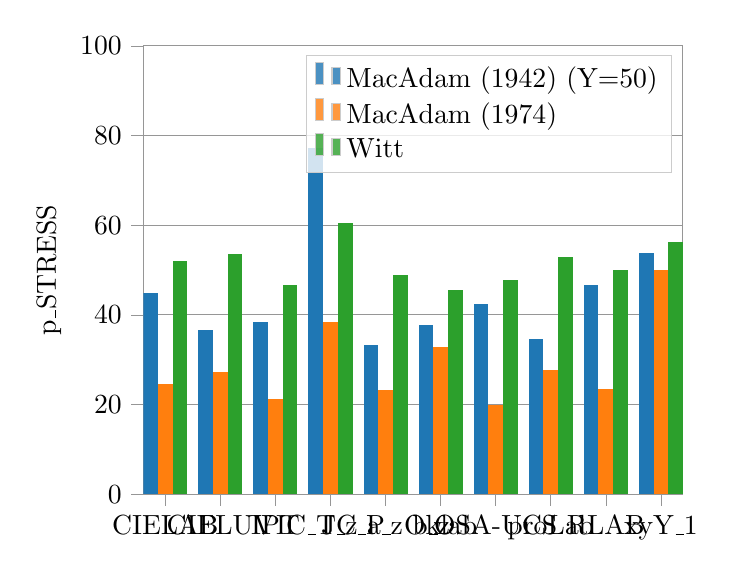
\begin{tikzpicture}

\definecolor{color0}{rgb}{0.12156862745098,0.466666666666667,0.705882352941177}
\definecolor{color1}{rgb}{1,0.498039215686275,0.0549019607843137}
\definecolor{color2}{rgb}{0.172549019607843,0.627450980392157,0.172549019607843}

\begin{axis}[
axis line style={white!58.8235294117647!black},
legend cell align={left},
legend style={fill opacity=0.8, draw opacity=1, text opacity=1, draw=white!80!black},
tick align=outside,
tick pos=left,
x grid style={white!58.8235294117647!black},
xmin=-0.4, xmax=9.4,
xtick style={color=white!58.8235294117647!black},
xtick={0,1,2,3,4,5,6,7,8,9},
xticklabels={CIELAB,CIELUV,IPT,IC\_TC\_P,J\_z a\_z b\_z,Oklab,OSA-UCS,proLab,RLAB,xyY\_1},
y grid style={white!58.8235294117647!black},
ylabel={p\_STRESS},
ymajorgrids,
ymin=0, ymax=100,
ytick style={color=white!58.8235294117647!black}
]
\draw[draw=none,fill=color0] (axis cs:-0.4,0) rectangle (axis cs:-0.133333333333333,44.8952155515788);
\addlegendimage{ybar,ybar legend,draw=none,fill=color0};
\addlegendentry{MacAdam (1942) (Y=50)}

\draw[draw=none,fill=color0] (axis cs:0.6,0) rectangle (axis cs:0.866666666666667,36.5010276032748);
\draw[draw=none,fill=color0] (axis cs:1.6,0) rectangle (axis cs:1.86666666666667,38.4833636095126);
\draw[draw=none,fill=color0] (axis cs:2.6,0) rectangle (axis cs:2.86666666666667,77.2316903365103);
\draw[draw=none,fill=color0] (axis cs:3.6,0) rectangle (axis cs:3.86666666666667,33.2757088119244);
\draw[draw=none,fill=color0] (axis cs:4.6,0) rectangle (axis cs:4.86666666666667,37.6772548200669);
\draw[draw=none,fill=color0] (axis cs:5.6,0) rectangle (axis cs:5.86666666666667,42.4396646797378);
\draw[draw=none,fill=color0] (axis cs:6.6,0) rectangle (axis cs:6.86666666666667,34.635501753967);
\draw[draw=none,fill=color0] (axis cs:7.6,0) rectangle (axis cs:7.86666666666667,46.581942046651);
\draw[draw=none,fill=color0] (axis cs:8.6,0) rectangle (axis cs:8.86666666666667,53.7506022511023);
\draw[draw=none,fill=color1] (axis cs:-0.133333333333333,0) rectangle (axis cs:0.133333333333333,24.5319191673876);
\addlegendimage{ybar,ybar legend,draw=none,fill=color1};
\addlegendentry{MacAdam (1974)}

\draw[draw=none,fill=color1] (axis cs:0.866666666666667,0) rectangle (axis cs:1.13333333333333,27.1465135470917);
\draw[draw=none,fill=color1] (axis cs:1.86666666666667,0) rectangle (axis cs:2.13333333333333,21.2696481498459);
\draw[draw=none,fill=color1] (axis cs:2.86666666666667,0) rectangle (axis cs:3.13333333333333,38.4505318024105);
\draw[draw=none,fill=color1] (axis cs:3.86666666666667,0) rectangle (axis cs:4.13333333333333,23.2111338532765);
\draw[draw=none,fill=color1] (axis cs:4.86666666666667,0) rectangle (axis cs:5.13333333333333,32.7178547285273);
\draw[draw=none,fill=color1] (axis cs:5.86666666666667,0) rectangle (axis cs:6.13333333333333,19.8475379525657);
\draw[draw=none,fill=color1] (axis cs:6.86666666666667,0) rectangle (axis cs:7.13333333333333,27.7092844635432);
\draw[draw=none,fill=color1] (axis cs:7.86666666666667,0) rectangle (axis cs:8.13333333333333,23.5028573394472);
\draw[draw=none,fill=color1] (axis cs:8.86666666666667,0) rectangle (axis cs:9.13333333333333,50.0184864244504);
\draw[draw=none,fill=color2] (axis cs:0.133333333333333,0) rectangle (axis cs:0.4,51.9845666548853);
\addlegendimage{ybar,ybar legend,draw=none,fill=color2};
\addlegendentry{Witt}

\draw[draw=none,fill=color2] (axis cs:1.13333333333333,0) rectangle (axis cs:1.4,53.5668514182667);
\draw[draw=none,fill=color2] (axis cs:2.13333333333333,0) rectangle (axis cs:2.4,46.7222778094553);
\draw[draw=none,fill=color2] (axis cs:3.13333333333333,0) rectangle (axis cs:3.4,60.5016229218686);
\draw[draw=none,fill=color2] (axis cs:4.13333333333333,0) rectangle (axis cs:4.4,48.8370743196918);
\draw[draw=none,fill=color2] (axis cs:5.13333333333333,0) rectangle (axis cs:5.4,45.4213412985957);
\draw[draw=none,fill=color2] (axis cs:6.13333333333333,0) rectangle (axis cs:6.4,47.6753713547588);
\draw[draw=none,fill=color2] (axis cs:7.13333333333333,0) rectangle (axis cs:7.4,52.78820194734);
\draw[draw=none,fill=color2] (axis cs:8.13333333333333,0) rectangle (axis cs:8.4,50.0899025149911);
\draw[draw=none,fill=color2] (axis cs:9.13333333333333,0) rectangle (axis cs:9.4,56.1591454267207);
\end{axis}

\end{tikzpicture}

\caption{$p_\text{STRESS}$ for a number of color spaces. The color space OSA-UCS was
designed specifically with the MacAdam \cite{macadam1974} dataset in mind. Both CAM
spaces perform well for all data sets. The MacAdam ellipses are assumed to exist without
  signficant change in a wide luminosity range, and is presented with $Y=50$ here.}
\end{figure}

\begin{figure}
\centering
  % This file was created by tikzplotlib v0.9.9.
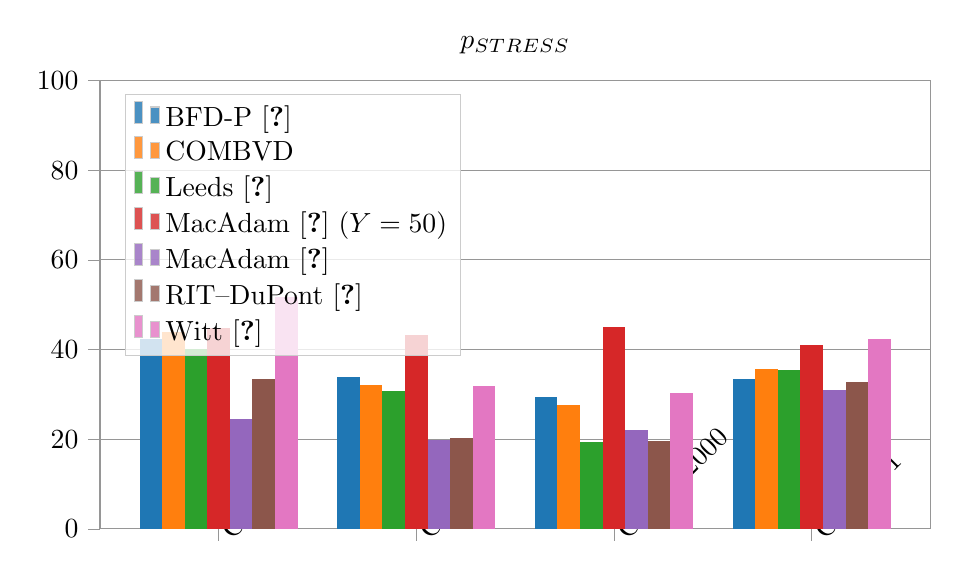
\begin{tikzpicture}

\definecolor{color0}{rgb}{0.12156862745098,0.466666666666667,0.705882352941177}
\definecolor{color1}{rgb}{1,0.498039215686275,0.0549019607843137}
\definecolor{color2}{rgb}{0.172549019607843,0.627450980392157,0.172549019607843}
\definecolor{color3}{rgb}{0.83921568627451,0.152941176470588,0.156862745098039}
\definecolor{color4}{rgb}{0.580392156862745,0.403921568627451,0.741176470588235}
\definecolor{color5}{rgb}{0.549019607843137,0.337254901960784,0.294117647058824}
\definecolor{color6}{rgb}{0.890196078431372,0.466666666666667,0.76078431372549}

\begin{axis}[
axis line style={white!58.8235294117647!black},
height=0.6\textwidth,
legend cell align={left},
legend style={
  fill opacity=0.8,
  draw opacity=1,
  text opacity=1,
  at={(0.03,0.97)},
  anchor=north west,
  draw=white!80!black
},
tick align=outside,
tick pos=left,
title={\(\displaystyle p_{STRESS}\)},
width=\textwidth,
x grid style={white!58.8235294117647!black},
xmin=-0.6, xmax=3.6,
xtick style={color=white!58.8235294117647!black},
xtick={0,1,2,3},
xticklabel style={rotate=45.0,anchor=west},
xticklabels={CIE76,CIE94,CIEDE2000,CMC 2:1},
y grid style={white!58.8235294117647!black},
ymajorgrids,
ymin=0, ymax=100,
ytick style={color=white!58.8235294117647!black}
]
\draw[draw=none,fill=color0] (axis cs:-0.4,0) rectangle (axis cs:-0.285714285714286,42.4095489785527);
\addlegendimage{ybar,ybar legend,draw=none,fill=color0}
\addlegendentry{BFD-P \cite{luorigg}}

\draw[draw=none,fill=color0] (axis cs:0.6,0) rectangle (axis cs:0.714285714285714,33.9166220461603);
\draw[draw=none,fill=color0] (axis cs:1.6,0) rectangle (axis cs:1.71428571428571,29.5212723042391);
\draw[draw=none,fill=color0] (axis cs:2.6,0) rectangle (axis cs:2.71428571428571,33.506587074841);
\draw[draw=none,fill=color1] (axis cs:-0.285714285714286,0) rectangle (axis cs:-0.171428571428571,43.9510829426371);
\addlegendimage{ybar,ybar legend,draw=none,fill=color1}
\addlegendentry{COMBVD}

\draw[draw=none,fill=color1] (axis cs:0.714285714285714,0) rectangle (axis cs:0.828571428571429,32.162114482167);
\draw[draw=none,fill=color1] (axis cs:1.71428571428571,0) rectangle (axis cs:1.82857142857143,27.5411916875731);
\draw[draw=none,fill=color1] (axis cs:2.71428571428571,0) rectangle (axis cs:2.82857142857143,35.7674847467488);
\draw[draw=none,fill=color2] (axis cs:-0.171428571428571,0) rectangle (axis cs:-0.0571428571428571,40.0364176602205);
\addlegendimage{ybar,ybar legend,draw=none,fill=color2}
\addlegendentry{Leeds \cite{leeds}}

\draw[draw=none,fill=color2] (axis cs:0.828571428571429,0) rectangle (axis cs:0.942857142857143,30.7398552375823);
\draw[draw=none,fill=color2] (axis cs:1.82857142857143,0) rectangle (axis cs:1.94285714285714,19.4609191829183);
\draw[draw=none,fill=color2] (axis cs:2.82857142857143,0) rectangle (axis cs:2.94285714285714,35.4800406903705);
\draw[draw=none,fill=color3] (axis cs:-0.0571428571428571,0) rectangle (axis cs:0.0571428571428571,44.8952155515788);
\addlegendimage{ybar,ybar legend,draw=none,fill=color3}
\addlegendentry{MacAdam \cite{macadam1942} ($Y=50$)}

\draw[draw=none,fill=color3] (axis cs:0.942857142857143,0) rectangle (axis cs:1.05714285714286,43.1638593810694);
\draw[draw=none,fill=color3] (axis cs:1.94285714285714,0) rectangle (axis cs:2.05714285714286,45.0506021909445);
\draw[draw=none,fill=color3] (axis cs:2.94285714285714,0) rectangle (axis cs:3.05714285714286,41.1259051595414);
\draw[draw=none,fill=color4] (axis cs:0.0571428571428571,0) rectangle (axis cs:0.171428571428571,24.5319191673876);
\addlegendimage{ybar,ybar legend,draw=none,fill=color4}
\addlegendentry{MacAdam \cite{macadam1974}}

\draw[draw=none,fill=color4] (axis cs:1.05714285714286,0) rectangle (axis cs:1.17142857142857,19.7853974310146);
\draw[draw=none,fill=color4] (axis cs:2.05714285714286,0) rectangle (axis cs:2.17142857142857,22.1289373697461);
\draw[draw=none,fill=color4] (axis cs:3.05714285714286,0) rectangle (axis cs:3.17142857142857,30.9828303427505);
\draw[draw=none,fill=color5] (axis cs:0.171428571428571,0) rectangle (axis cs:0.285714285714286,33.364735317963);
\addlegendimage{ybar,ybar legend,draw=none,fill=color5}
\addlegendentry{RIT--DuPont \cite{berns}}

\draw[draw=none,fill=color5] (axis cs:1.17142857142857,0) rectangle (axis cs:1.28571428571429,20.3557004987779);
\draw[draw=none,fill=color5] (axis cs:2.17142857142857,0) rectangle (axis cs:2.28571428571429,19.5111243169988);
\draw[draw=none,fill=color5] (axis cs:3.17142857142857,0) rectangle (axis cs:3.28571428571429,32.8046660031734);
\draw[draw=none,fill=color6] (axis cs:0.285714285714286,0) rectangle (axis cs:0.4,51.6740349454926);
\addlegendimage{ybar,ybar legend,draw=none,fill=color6}
\addlegendentry{Witt \cite{witt}}

\draw[draw=none,fill=color6] (axis cs:1.28571428571429,0) rectangle (axis cs:1.4,31.9666655304065);
\draw[draw=none,fill=color6] (axis cs:2.28571428571429,0) rectangle (axis cs:2.4,30.369462501181);
\draw[draw=none,fill=color6] (axis cs:3.28571428571429,0) rectangle (axis cs:3.4,42.3944471199168);
\end{axis}

\end{tikzpicture}

  \caption{$p_\text{STRESS}$ for a number of color diffence formulae.
  CIE76 is really just the Euclidean distance in CIELAB, the other difference formulas
  are non-Euclidean.}
\end{figure}

A common special case of this setting is distance data given in terms of ellipse points,
i.e., a color center with a number of standard deviations (or similar) in various
directions. The famous MacAdam ellipses \cite{macadam1942} are derived from such data.
Since the ellipses are supposed to to be circles of equal size in the transformed space,
the target value for all $d_i$ is 1. The parameter $\alpha$ simplifies to be the average
over all $\delta_i$ and we have
\begin{equation}\label{eq:e}
  e_{\text{STRESS}}
  \coloneqq
  100
  \frac{%
    \sqrt{\sum_{i=1}^n (\alpha - \delta_{i})^2}
  }{
    \sqrt{\sum_{i=1}^n \delta_i^2}
  }.
\end{equation}
In case only the actual ellipses are given (e.g., \cite{luorigg}), one can place a
number of points onto their boundaries (e.g., 8 or 16) and compute the residual with
from them.

\begin{remark}
  While the generation of ellipses from experimental data is useful for visually
  representing color difference data, there are a number of criticisms associated with
  using them in color space evaluation and optimization.
  \begin{itemize}
    \item Ellipses encode the raw experimental data, and perhaps distort it in some way.
      If experimental data is available, using it directly eliminates this layer of
      distortion.
    \item When calculating the STRESS of ellipse data, one has to choose a set of points
      on each ellipse and compute the STRESS for the distances. The final value depends
      on how many values where chosen and where they sit on the ellipses.
    \item Ellipses are two-dimensional geometric objects while color spaces are
      three-dimensional. In many cases, ellipses are drawn orthogonal to the perceived
      lightness dimension, and hence contain no information about lightness, even if the
      original data did.
    \item In some cases, e.g., \cite{macadam1942}, only the chromaticity coordinates $x$
      and $y$ are given for the ellipses, not the lightness component $Y$. The claim is
      that the ellipses don't change signficantly between different levels of lightness
      \cite{brown}. However, this is true at most in a particular range of luminosity
      which is often not provided.
    \end{itemize}
\end{remark}


\subsection{Cost functional for hue linearity}

\begin{figure}
  \centering
  % This file was created with tikzplotlib v0.9.11.
\begin{tikzpicture}

\begin{axis}[
tick align=outside,
tick pos=left,
ticks=none,
title={XYY},
width=0.39\textwidth,
x grid style={white!69.0196078431373!black},
xlabel={x},
xmin=0.119853419956019, xmax=0.643318261961687,
xtick style={color=black},
y grid style={white!69.0196078431373!black},
ylabel style={rotate=-90.0},
ylabel={y},
ymin=0.051747422449696, ymax=0.636002979799659,
ytick style={color=black}
]
\addplot [semithick, gray]
table {%
0.310060511024135 0.316149551383787
0.618510782465492 0.359524123377867
};
\addplot [semithick, gray]
table {%
0.310060511024135 0.316149551383787
0.492805485084296 0.450964897591934
};
\addplot [semithick, gray]
table {%
0.310060511024135 0.316149551383787
0.425845205623366 0.49947312734917
};
\addplot [semithick, gray]
table {%
0.310060511024135 0.316149551383787
0.373114155681491 0.539497615223761
};
\addplot [semithick, gray]
table {%
0.310060511024135 0.316149551383787
0.287216983469216 0.609445909011024
};
\addplot [semithick, gray]
table {%
0.310060511024135 0.316149551383787
0.22737797418911 0.382732622800503
};
\addplot [semithick, gray]
table {%
0.310060511024135 0.316149551383787
0.209349676200864 0.304924341509052
};
\addplot [semithick, gray]
table {%
0.310060511024135 0.316149551383787
0.189844060535908 0.237486274034248
};
\addplot [semithick, gray]
table {%
0.310060511024135 0.316149551383787
0.143647276410822 0.0878670043500509
};
\addplot [semithick, gray]
table {%
0.310060511024135 0.316149551383787
0.263191431588283 0.132669856355077
};
\addplot [semithick, gray]
table {%
0.310060511024135 0.316149551383787
0.33161599834101 0.174382451500175
};
\addplot [semithick, gray]
table {%
0.310060511024135 0.316149551383787
0.415156388774311 0.226490214166486
};
\addplot [
  mark=*,
  only marks,
  scatter,
  scatter/@post marker code/.code={%
  \endscope
},
  scatter/@pre marker code/.code={%
  \expanded{%
  \noexpand\definecolor{thispointdrawcolor}{RGB}{\drawcolor}%
  \noexpand\definecolor{thispointfillcolor}{RGB}{\fillcolor}%
  }%
  \scope[draw=thispointdrawcolor, fill=thispointfillcolor]%
},
  visualization depends on={value \thisrow{draw} \as \drawcolor},
  visualization depends on={value \thisrow{fill} \as \fillcolor}
]
table [search path={./figures/}]{hung-berns-xyy-000.dat};
\end{axis}

\end{tikzpicture}

  \hfill
  % This file was created with tikzplotlib v0.9.11.
\begin{tikzpicture}

\begin{axis}[
tick align=outside,
tick pos=left,
ticks=none,
title={CIELAB},
width=0.39\textwidth,
x grid style={white!69.0196078431373!black},
xlabel={a*},
xmin=-108.564286272053, xmax=101.03048079993,
xtick style={color=black},
y grid style={white!69.0196078431373!black},
ylabel style={rotate=-90.0},
ylabel={b*},
ymin=-118.387351085463, ymax=107.427562033836,
ytick style={color=black}
]
\addplot [semithick, gray]
table {%
5.25252896445825 -5.56774961768019
80.6478891890955 75.0003676704183
};
\addplot [semithick, gray]
table {%
5.25252896445825 -5.56774961768019
21.6509757498035 86.7199588588502
};
\addplot [semithick, gray]
table {%
5.25252896445825 -5.56774961768019
-20.0745782448384 96.4047384194088
};
\addplot [semithick, gray]
table {%
5.25252896445825 -5.56774961768019
-53.0285304224634 90.2168087210625
};
\addplot [semithick, gray]
table {%
5.25252896445825 -5.56774961768019
-99.0372514051445 81.8748620664602
};
\addplot [semithick, gray]
table {%
5.25252896445825 -5.56774961768019
-68.5339408040773 4.43655416117572
};
\addplot [semithick, gray]
table {%
5.25252896445825 -5.56774961768019
-46.0910964425066 -24.679439217135
};
\addplot [semithick, gray]
table {%
5.25252896445825 -5.56774961768019
-20.4072010476058 -46.379560524849
};
\addplot [semithick, gray]
table {%
5.25252896445825 -5.56774961768019
57.8416360574993 -108.123036852768
};
\addplot [semithick, gray]
table {%
5.25252896445825 -5.56774961768019
81.5579277515681 -74.7653944932216
};
\addplot [semithick, gray]
table {%
5.25252896445825 -5.56774961768019
91.5034459330218 -53.4221278151268
};
\addplot [semithick, gray]
table {%
5.25252896445825 -5.56774961768019
84.7374719579833 -17.6689957255866
};
\addplot [
  mark=*,
  only marks,
  scatter,
  scatter/@post marker code/.code={%
  \endscope
},
  scatter/@pre marker code/.code={%
  \expanded{%
  \noexpand\definecolor{thispointdrawcolor}{RGB}{\drawcolor}%
  \noexpand\definecolor{thispointfillcolor}{RGB}{\fillcolor}%
  }%
  \scope[draw=thispointdrawcolor, fill=thispointfillcolor]%
},
  visualization depends on={value \thisrow{draw} \as \drawcolor},
  visualization depends on={value \thisrow{fill} \as \fillcolor}
]
table [search path={./figures/}]{hung-berns-cielab-000.dat};
\end{axis}

\end{tikzpicture}

  \hfill
  % This file was created with tikzplotlib v0.9.12.
\begin{tikzpicture}

\begin{axis}[
tick align=outside,
tick pos=left,
ticks=none,
title={OKLAB},
width=0.39\textwidth,
x grid style={white!69.0196078431373!black},
xlabel={a},
xmin=-0.288307512005136, xmax=0.286141954639072,
xtick style={color=black},
y grid style={white!69.0196078431373!black},
ylabel style={rotate=-90.0},
ylabel={b},
ymin=-0.322127479094392, ymax=0.228811043834133,
ytick style={color=black}
]
\addplot [semithick, gray]
table {%
0.0137565554683805 -0.0148789811996328
0.214596337211429 0.143591784000024
};
\addplot [semithick, gray]
table {%
0.0137565554683805 -0.0148789811996328
0.0514852487639785 0.176292155547739
};
\addplot [semithick, gray]
table {%
0.0137565554683805 -0.0148789811996328
-0.0595662853089172 0.203544635881957
};
\addplot [semithick, gray]
table {%
0.0137565554683805 -0.0148789811996328
-0.145832522001159 0.195775092575124
};
\addplot [semithick, gray]
table {%
0.0137565554683805 -0.0148789811996328
-0.260889697777951 0.182855649831706
};
\addplot [semithick, gray]
table {%
0.0137565554683805 -0.0148789811996328
-0.194003195692591 0.010404680847883
};
\addplot [semithick, gray]
table {%
0.0137565554683805 -0.0148789811996328
-0.154031014673414 -0.0690988040380578
};
\addplot [semithick, gray]
table {%
0.0137565554683805 -0.0148789811996328
-0.108206416192123 -0.133629409466217
};
\addplot [semithick, gray]
table {%
0.0137565554683805 -0.0148789811996328
-0.0390112196334746 -0.294073449729041
};
\addplot [semithick, gray]
table {%
0.0137565554683805 -0.0148789811996328
0.191230633092283 -0.208650835956893
};
\addplot [semithick, gray]
table {%
0.0137565554683805 -0.0148789811996328
0.257719185584806 -0.146344775121726
};
\addplot [semithick, gray]
table {%
0.0137565554683805 -0.0148789811996328
0.259562150573521 -0.0463907316188274
};
\addplot [
  mark=*,
  only marks,
  scatter,
  scatter/@post marker code/.code={%
  \endscope
},
  scatter/@pre marker code/.code={%
  \expanded{%
  \noexpand\definecolor{thispointdrawcolor}{RGB}{\drawcolor}%
  \noexpand\definecolor{thispointfillcolor}{RGB}{\fillcolor}%
  }%
  \scope[draw=thispointdrawcolor, fill=thispointfillcolor]%
},
  visualization depends on={value \thisrow{draw} \as \drawcolor},
  visualization depends on={value \thisrow{fill} \as \fillcolor}
]
table [search path={./figures/}]{hung-berns-oklab-000.dat};
\end{axis}

\end{tikzpicture}

  \caption{Hung-Berns \cite{hung} hue linearity data for three color spaces. The points
  which are representable in sRGB are shown in color.}
\end{figure}

There are multiple experiments about which colors are perceived to be of equal
hue~\cite{hung,ebner,xiao} (see figure~\ref{fig:hstress}). Color spaces are considered
good if the transformation maps points of equal perceived hue onto a straight line.

What is a good measure of how well points sit on a straight line?
A common idea is to find the straight line that mimizes the sum of squared distances to
all points. This general approach is referred to as \emph{total least squares (TLS)}.
The line is typically
given implicitly by $\alpha_1 x + \alpha_2 y
= 0$ with $\alpha_1,\alpha_2\in\R$, $\|\alpha\|_2^2 = \alpha_1^2 + \alpha_2^2 = 1$.
Because this assumes that the line passes through the origin, all points are
first translated such that the whitepoint sits in in origin.
For scale-invariance, it is convenient to divide by the maximizer of the squared
distances, in total:
\begin{equation}\label{eq:l}
h_2 \coloneqq
  \frac{
\min_{\|\alpha\|_2=1}
  \sqrt{\sum_{i=1}^n (\alpha_1 \tilde{x}_i + \alpha_2 \tilde{y}_i)^2}
}{
\max_{\|\alpha\|_2=1}
  \sqrt{\sum_{i=1}^n (\alpha_1 \tilde{x}_i + \alpha_2 \tilde{y}_i)^2}
}
\end{equation}
with the translated sample points
\[
  \tilde{x}_i \coloneqq x_i-w_x,\qquad
  \tilde{y}_i \coloneqq y_i-w_y.
\]
The value of $h_2$ can be approximated with any appropriate optimization method. A more
explicit and more easily computable representation however is retrieved as follows.
With the $n$-by-2 coordinate matrix
\[
  A \coloneqq \begin{pmatrix}
    \tilde{x}_1 & \tilde{y}_1\\
    \vdots & \vdots\\
    \tilde{x}_n & \tilde{y}_n
  \end{pmatrix},
\]
the sum in \eqref{eq:l} can be written as
\[
  \sum_{i=1}^n (\alpha_1 \tilde{x}_i + \alpha_2 \tilde{y}_i)^2
  = (A \alpha)^T (A \alpha)
  = \alpha^T A^T A \alpha.
\]
This makes clear that $h_2$ is exactly the ratio of the square roots of the two
eigenvalues of $A^TA$ or equivalently the ratio of the two singular values of $A$,
\[
h_2
= \frac{
  \sqrt{\lambda_{\min}(A^T A)}
  }{
    \sqrt{\lambda_{\max}(A^T A)}
  }
= \frac{\sigma_{\min}(A)}{\sigma_{\max}(A)}.
\]
The value is given explicitly by
\begin{equation*}
  h_2 = \sqrt{
    \frac{
      \xt^T\xt
      + \yt^T\yt
      - \sqrt{(\xt^T\xt - \yt^T\yt)^2 + 4 (\xt^T\yt)^2}
    }{
      \xt^T\xt
      + \yt^T\yt
      + \sqrt{(\xt^T\xt - \yt^T\yt)^2 + 4 (\xt^T\yt)^2}
    }
    }.
\end{equation*}
The expression under the outer root is indeed always nonnegative by virtue of the
Cauchy-Schwarz inequality $(\xt^T\yt)^2 \le (\xt^T\xt) (\yt^T\yt)$. It is 0 if and only
if $\xt$ and $\yt$ are linearly dependent, i.e., if the points $(x_i, y_i)$ sit on a
straight line through the origin.

Since $0\le h_2\le 1$, the value can be given in terms of STRESS,
\begin{equation}\label{eq:hstress}
  h_\text{STRESS} = 100 \frac{\sigma_{\min}(A)}{\sigma_{\max}(A)}.
\end{equation}


% \begin{remark}
%   The representation \eqref{eq:s2} is suitable for optimization purposes. Since a value
%   $\sqrt{t}$ is small if and only if $t$ is small, one would in the interest of
%   simplicity disregard the outer square root.
% \end{remark}


\begin{figure}
  \centering
  % This file was created with tikzplotlib v0.9.12.
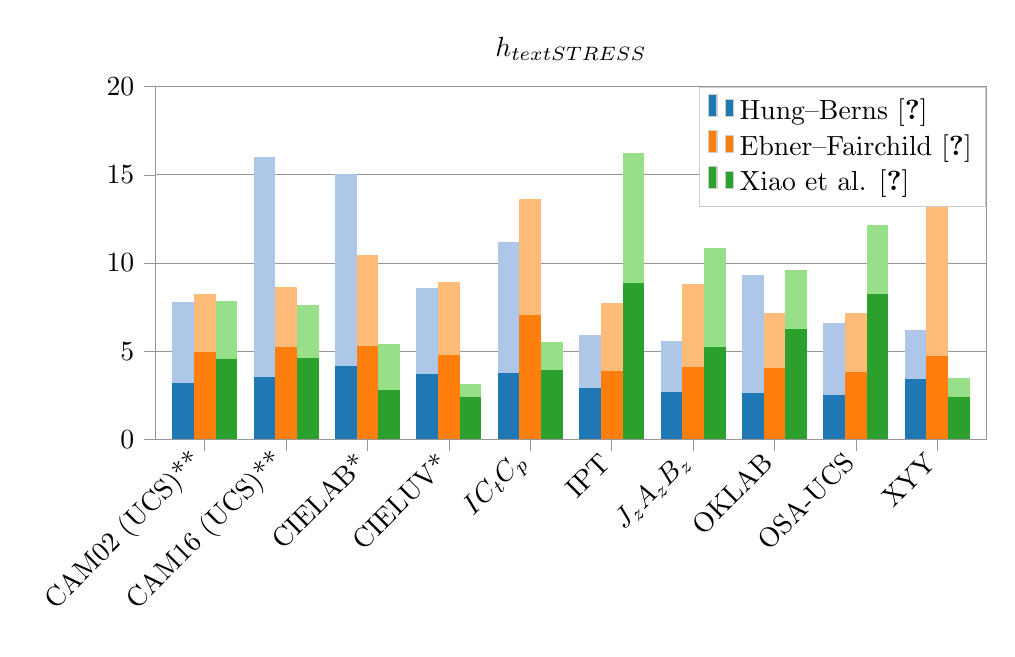
\begin{tikzpicture}

\definecolor{color0}{rgb}{0.12156862745098,0.466666666666667,0.705882352941177}
\definecolor{color1}{rgb}{0.682352941176471,0.780392156862745,0.909803921568627}
\definecolor{color2}{rgb}{1,0.498039215686275,0.0549019607843137}
\definecolor{color3}{rgb}{1,0.733333333333333,0.470588235294118}
\definecolor{color4}{rgb}{0.172549019607843,0.627450980392157,0.172549019607843}
\definecolor{color5}{rgb}{0.596078431372549,0.874509803921569,0.541176470588235}

\begin{axis}[
axis line style={white!58.8235294117647!black},
height=0.5\textwidth,
legend cell align={left},
legend style={fill opacity=1, draw opacity=1, text opacity=1, at={(1,1)}, draw=white!80!black},
tick align=outside,
tick pos=left,
title={\(\displaystyle h_{text{STRESS}}\)},
width=\textwidth,
x grid style={white!58.8235294117647!black},
xmin=-0.6, xmax=9.6,
xtick style={color=white!58.8235294117647!black},
xtick={0,1,2,3,4,5,6,7,8,9},
xticklabel style={rotate=45.0,anchor=east},
xticklabels={
  CAM02 (UCS)**,
  CAM16 (UCS)**,
  CIELAB*,
  CIELUV*,
  \(\displaystyle IC_tC_p\),
  IPT,
  \(\displaystyle J_zA_zB_z\),
  OKLAB,
  OSA-UCS,
  XYY
},
y grid style={white!58.8235294117647!black},
ymajorgrids,
ymin=0, ymax=20,
ytick style={color=white!58.8235294117647!black},
ytick={0,5,10,15,20}
]
\draw[draw=none,fill=color0] (axis cs:-0.4,0) rectangle (axis cs:-0.133333333333333,3.18845620008038);
\addlegendimage{ybar,ybar legend,draw=none,fill=color0}
\addlegendentry{Hung--Berns \cite{hung}}

\draw[draw=none,fill=color0] (axis cs:0.6,0) rectangle (axis cs:0.866666666666667,3.52855078191527);
\draw[draw=none,fill=color0] (axis cs:1.6,0) rectangle (axis cs:1.86666666666667,4.14821469192855);
\draw[draw=none,fill=color0] (axis cs:2.6,0) rectangle (axis cs:2.86666666666667,3.69928776179375);
\draw[draw=none,fill=color0] (axis cs:3.6,0) rectangle (axis cs:3.86666666666667,3.79577398935562);
\draw[draw=none,fill=color0] (axis cs:4.6,0) rectangle (axis cs:4.86666666666667,2.92119683105357);
\draw[draw=none,fill=color0] (axis cs:5.6,0) rectangle (axis cs:5.86666666666667,2.68536426894408);
\draw[draw=none,fill=color0] (axis cs:6.6,0) rectangle (axis cs:6.86666666666667,2.63371950519243);
\draw[draw=none,fill=color0] (axis cs:7.6,0) rectangle (axis cs:7.86666666666667,2.49530998013144);
\draw[draw=none,fill=color0] (axis cs:8.6,0) rectangle (axis cs:8.86666666666667,3.44018748653443);
\draw[draw=none,fill=color1] (axis cs:-0.4,3.18845620008038) rectangle (axis cs:-0.133333333333333,7.77803913385343);
\draw[draw=none,fill=color1] (axis cs:0.6,3.52855078191527) rectangle (axis cs:0.866666666666667,16.0323471051899);
\draw[draw=none,fill=color1] (axis cs:1.6,4.14821469192855) rectangle (axis cs:1.86666666666667,15.0311575636155);
\draw[draw=none,fill=color1] (axis cs:2.6,3.69928776179375) rectangle (axis cs:2.86666666666667,8.56391940890914);
\draw[draw=none,fill=color1] (axis cs:3.6,3.79577398935562) rectangle (axis cs:3.86666666666667,11.1890830346538);
\draw[draw=none,fill=color1] (axis cs:4.6,2.92119683105357) rectangle (axis cs:4.86666666666667,5.89478443004318);
\draw[draw=none,fill=color1] (axis cs:5.6,2.68536426894408) rectangle (axis cs:5.86666666666667,5.55970441646704);
\draw[draw=none,fill=color1] (axis cs:6.6,2.63371950519243) rectangle (axis cs:6.86666666666667,9.31997777958701);
\draw[draw=none,fill=color1] (axis cs:7.6,2.49530998013144) rectangle (axis cs:7.86666666666667,6.59231944961339);
\draw[draw=none,fill=color1] (axis cs:8.6,3.44018748653443) rectangle (axis cs:8.86666666666667,6.18717018996993);
\draw[draw=none,fill=color2] (axis cs:-0.133333333333333,0) rectangle (axis cs:0.133333333333333,4.96820230766771);
\addlegendimage{ybar,ybar legend,draw=none,fill=color2}
\addlegendentry{Ebner--Fairchild \cite{ebner}}

\draw[draw=none,fill=color2] (axis cs:0.866666666666667,0) rectangle (axis cs:1.13333333333333,5.25888517471055);
\draw[draw=none,fill=color2] (axis cs:1.86666666666667,0) rectangle (axis cs:2.13333333333333,5.29206832728103);
\draw[draw=none,fill=color2] (axis cs:2.86666666666667,0) rectangle (axis cs:3.13333333333333,4.81360584972163);
\draw[draw=none,fill=color2] (axis cs:3.86666666666667,0) rectangle (axis cs:4.13333333333333,7.04859738515829);
\draw[draw=none,fill=color2] (axis cs:4.86666666666667,0) rectangle (axis cs:5.13333333333333,3.8585452834895);
\draw[draw=none,fill=color2] (axis cs:5.86666666666667,0) rectangle (axis cs:6.13333333333333,4.11463844120849);
\draw[draw=none,fill=color2] (axis cs:6.86666666666667,0) rectangle (axis cs:7.13333333333333,4.05730886560147);
\draw[draw=none,fill=color2] (axis cs:7.86666666666667,0) rectangle (axis cs:8.13333333333333,3.81297237590754);
\draw[draw=none,fill=color2] (axis cs:8.86666666666667,0) rectangle (axis cs:9.13333333333333,4.75045818919245);
\draw[draw=none,fill=color3] (axis cs:-0.133333333333333,4.96820230766771) rectangle (axis cs:0.133333333333333,8.22072308329214);
\draw[draw=none,fill=color3] (axis cs:0.866666666666667,5.25888517471055) rectangle (axis cs:1.13333333333333,8.66022068747131);
\draw[draw=none,fill=color3] (axis cs:1.86666666666667,5.29206832728103) rectangle (axis cs:2.13333333333333,10.4569873793138);
\draw[draw=none,fill=color3] (axis cs:2.86666666666667,4.81360584972163) rectangle (axis cs:3.13333333333333,8.91448406046236);
\draw[draw=none,fill=color3] (axis cs:3.86666666666667,7.04859738515829) rectangle (axis cs:4.13333333333333,13.6280487760657);
\draw[draw=none,fill=color3] (axis cs:4.86666666666667,3.8585452834895) rectangle (axis cs:5.13333333333333,7.72233957150083);
\draw[draw=none,fill=color3] (axis cs:5.86666666666667,4.11463844120849) rectangle (axis cs:6.13333333333333,8.80555808427234);
\draw[draw=none,fill=color3] (axis cs:6.86666666666667,4.05730886560147) rectangle (axis cs:7.13333333333333,7.16171792324175);
\draw[draw=none,fill=color3] (axis cs:7.86666666666667,3.81297237590754) rectangle (axis cs:8.13333333333333,7.17861133082468);
\draw[draw=none,fill=color3] (axis cs:8.86666666666667,4.75045818919245) rectangle (axis cs:9.13333333333333,13.4354916910975);
\draw[draw=none,fill=color4] (axis cs:0.133333333333333,0) rectangle (axis cs:0.4,4.58825706817218);
\addlegendimage{ybar,ybar legend,draw=none,fill=color4}
\addlegendentry{Xiao et al. \cite{xiao}}

\draw[draw=none,fill=color4] (axis cs:1.13333333333333,0) rectangle (axis cs:1.4,4.62695701852859);
\draw[draw=none,fill=color4] (axis cs:2.13333333333333,0) rectangle (axis cs:2.4,2.78836260423616);
\draw[draw=none,fill=color4] (axis cs:3.13333333333333,0) rectangle (axis cs:3.4,2.38128547870168);
\draw[draw=none,fill=color4] (axis cs:4.13333333333333,0) rectangle (axis cs:4.4,3.92409485524028);
\draw[draw=none,fill=color4] (axis cs:5.13333333333333,0) rectangle (axis cs:5.4,8.85387808189672);
\draw[draw=none,fill=color4] (axis cs:6.13333333333333,0) rectangle (axis cs:6.4,5.2305294695945);
\draw[draw=none,fill=color4] (axis cs:7.13333333333333,0) rectangle (axis cs:7.4,6.25638644449191);
\draw[draw=none,fill=color4] (axis cs:8.13333333333333,0) rectangle (axis cs:8.4,8.22761086694145);
\draw[draw=none,fill=color4] (axis cs:9.13333333333333,0) rectangle (axis cs:9.4,2.3985002202066);
\draw[draw=none,fill=color5] (axis cs:0.133333333333333,4.58825706817218) rectangle (axis cs:0.4,7.8366298874709);
\draw[draw=none,fill=color5] (axis cs:1.13333333333333,4.62695701852859) rectangle (axis cs:1.4,7.63990114805117);
\draw[draw=none,fill=color5] (axis cs:2.13333333333333,2.78836260423616) rectangle (axis cs:2.4,5.41428572442929);
\draw[draw=none,fill=color5] (axis cs:3.13333333333333,2.38128547870168) rectangle (axis cs:3.4,3.13325181065191);
\draw[draw=none,fill=color5] (axis cs:4.13333333333333,3.92409485524028) rectangle (axis cs:4.4,5.52652985033793);
\draw[draw=none,fill=color5] (axis cs:5.13333333333333,8.85387808189672) rectangle (axis cs:5.4,16.2208566981952);
\draw[draw=none,fill=color5] (axis cs:6.13333333333333,5.2305294695945) rectangle (axis cs:6.4,10.855292125204);
\draw[draw=none,fill=color5] (axis cs:7.13333333333333,6.25638644449191) rectangle (axis cs:7.4,9.59481014620975);
\draw[draw=none,fill=color5] (axis cs:8.13333333333333,8.22761086694145) rectangle (axis cs:8.4,12.1368913781661);
\draw[draw=none,fill=color5] (axis cs:9.13333333333333,2.3985002202066) rectangle (axis cs:9.4,3.47049524917497);
\end{axis}

\end{tikzpicture}

  \caption{$h_\text{STRESS}$ for different data sets. The darker bar represents the
  average $h_\text{STRESS}$ over all arms in the data set ($M_1$), the light bar
  indicates the maximum ($M_{\infty}$).  The largest maxima are CIELAB's and CAM16's
  famous nonlinearities for blue.
  $J_za_zb_z$ and Oklab perform best for all data sets.}
  \label{fig:hstress}
\end{figure}

\subsection{Cost functional for lightness data}

\begin{figure}
  \centering
  % This file was created by tikzplotlib v0.9.9.
\begin{tikzpicture}
\scriptsize

\definecolor{color0}{rgb}{0.12156862745098,0.466666666666667,0.705882352941177}
\definecolor{color1}{rgb}{1,0.498039215686275,0.0549019607843137}

\begin{axis}[
axis line style={white!58.8235294117647!black},
height=0.3\textwidth,
tick align=outside,
tick pos=left,
title={CIELAB},
width=0.33\textwidth,
x grid style={white!58.8235294117647!black},
xlabel={Y},
xmin=0, xmax=102.56,
xtick style={color=white!58.8235294117647!black},
y grid style={white!58.8235294117647!black},
ylabel style={rotate=-90.0},
ylabel={L*},
ymajorgrids,
ymin=0, ymax=102.235748429383,
ytick style={color=white!58.8235294117647!black}
]
\addplot [semithick, color0]
table [search path={./figures/}] {munsell-lightness-cielab-000.dat};
\path [draw=color1, semithick]
(axis cs:1.21,10.6309369261204)
--(axis cs:1.21,10.6309369261204);

\path [draw=color1, semithick]
(axis cs:3.126,20.5416073870883)
--(axis cs:3.126,20.5416073870883);

\path [draw=color1, semithick]
(axis cs:6.555,30.7715993950525)
--(axis cs:6.555,30.7715993950525);

\path [draw=color1, semithick]
(axis cs:12,41.2161201244669)
--(axis cs:12,41.2161201244669);

\path [draw=color1, semithick]
(axis cs:19.77,51.5761656343387)
--(axis cs:19.77,51.5761656343387);

\path [draw=color1, semithick]
(axis cs:30.05,61.6973394989073)
--(axis cs:30.05,61.6973394989073);

\path [draw=color1, semithick]
(axis cs:43.06,71.5956751616161)
--(axis cs:43.06,71.5956751616161);

\path [draw=color1, semithick]
(axis cs:59.1,81.3465316853443)
--(axis cs:59.1,81.3465316853443);

\path [draw=color1, semithick]
(axis cs:78.66,91.0802319490308)
--(axis cs:78.66,91.0802319490308);

\addplot [semithick, color1, mark=*, mark size=3, mark options={solid}, only marks]
table [search path={./figures/}] {munsell-lightness-cielab-001.dat};
\end{axis}

\end{tikzpicture}

  \hfill
  % This file was created by tikzplotlib v0.9.9.
\begin{tikzpicture}
\scriptsize

\definecolor{color0}{rgb}{0.12156862745098,0.466666666666667,0.705882352941177}
\definecolor{color1}{rgb}{1,0.498039215686275,0.0549019607843137}

\begin{axis}[
axis line style={white!58.8235294117647!black},
height=0.3\textwidth,
tick align=outside,
tick pos=left,
title={IPT},
width=0.33\textwidth,
x grid style={white!58.8235294117647!black},
xlabel={Y},
xmin=0, xmax=102.56,
xtick style={color=white!58.8235294117647!black},
y grid style={white!58.8235294117647!black},
ylabel style={rotate=-90.0},
ylabel={I},
ymajorgrids,
ymin=0, ymax=7.18187462223965,
ytick style={color=white!58.8235294117647!black}
]
\addplot [semithick, color0]
table [search path={./figures/}] {munsell-lightness-ipt-000.dat};
\path [draw=color1, semithick]
(axis cs:1.21,0.919189723601696)
--(axis cs:1.21,2.18028435365019);

\path [draw=color1, semithick]
(axis cs:3.126,1.35036487591379)
--(axis cs:3.126,2.69422770146139);

\path [draw=color1, semithick]
(axis cs:6.555,1.86440469480022)
--(axis cs:6.555,3.26591888412707);

\path [draw=color1, semithick]
(axis cs:12,2.40417588868152)
--(axis cs:12,3.86208817235529);

\path [draw=color1, semithick]
(axis cs:19.77,2.95098814706442)
--(axis cs:19.77,4.42054177606006);

\path [draw=color1, semithick]
(axis cs:30.05,3.52440771467503)
--(axis cs:30.05,4.96696794127002);

\path [draw=color1, semithick]
(axis cs:43.06,4.15853254448133)
--(axis cs:43.06,5.56389163621633);

\path [draw=color1, semithick]
(axis cs:59.1,4.69394682727128)
--(axis cs:59.1,6.1478586806875);

\path [draw=color1, semithick]
(axis cs:78.66,5.45545216758606)
--(axis cs:78.66,6.73670858328733);

\addplot [semithick, color1, mark=*, mark size=3, mark options={solid}, only marks]
table [search path={./figures/}] {munsell-lightness-ipt-001.dat};
\end{axis}

\end{tikzpicture}

  \hfill
  % This file was created by tikzplotlib v0.9.7.
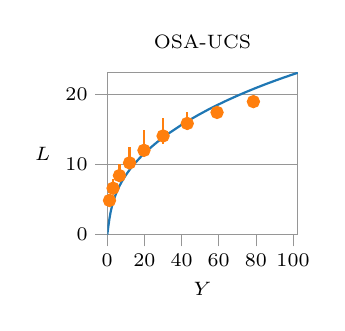
\begin{tikzpicture}
\scriptsize

\definecolor{color0}{rgb}{1,0.498039215686275,0.0549019607843137}
\definecolor{color1}{rgb}{0.12156862745098,0.466666666666667,0.705882352941177}

\begin{axis}[
axis line style={white!58.8235294117647!black},
height=0.3\textwidth,
tick align=outside,
tick pos=left,
title={OSA-UCS},
width=0.33\textwidth,
x grid style={white!58.8235294117647!black},
xlabel={$Y$},
xmin=0, xmax=102.56,
xtick style={color=white!58.8235294117647!black},
y grid style={white!58.8235294117647!black},
ylabel style={rotate=-90.0},
ylabel={$L$},
ymajorgrids,
ymin=0, ymax=23.0677681912702,
ytick style={color=white!58.8235294117647!black},
yticklabel style={anchor=east}
]
\path [draw=color0, thick]
(axis cs:1.21,4.35547008975803)
--(axis cs:1.21,5.45909323297212);

\path [draw=color0, thick]
(axis cs:3.126,5.94716408570973)
--(axis cs:3.126,7.86657831058072);

\path [draw=color0, thick]
(axis cs:6.555,7.63098727912685)
--(axis cs:6.555,10.1386880703995);

\path [draw=color0, thick]
(axis cs:12,9.35970227039494)
--(axis cs:12,12.4343457671405);

\path [draw=color0, thick]
(axis cs:19.77,11.113588693241)
--(axis cs:19.77,14.9477695878852);

\path [draw=color0, thick]
(axis cs:30.05,12.9125629677715)
--(axis cs:30.05,16.572351079197);

\path [draw=color0, thick]
(axis cs:43.06,15.1294134600825)
--(axis cs:43.06,17.447699260164);

\path [draw=color0, thick]
(axis cs:59.1,16.8410538607205)
--(axis cs:59.1,18.5262074576843);

\path [draw=color0, thick]
(axis cs:78.66,18.5247996733385)
--(axis cs:78.66,19.469531790342);

\addplot [thick, color1]
table {%
0 0
0.375 0.738168597221375
0.580999970436096 1.15338838100433
1.03400003910065 2.00689578056335
1.23800003528595 2.35291242599487
1.68099999427795 3.02187752723694
1.75199997425079 3.11414861679077
1.9650000333786 3.39096188545227
2.13599991798401 3.59857177734375
2.46499991416931 3.96765613555908
2.8050000667572 4.31367254257202
3.15199995040894 4.63662147521973
3.50099992752075 4.93650245666504
3.87700009346008 5.23638343811035
4.25 5.51319646835327
4.61399984359741 5.76694202423096
5.03599977493286 6.04375505447388
5.40799999237061 6.27443313598633
6.08599996566772 6.66658496856689
6.73099994659424 7.01260137557983
7.4229998588562 7.35861825942993
8.11100006103516 7.68156671524048
8.89500045776367 8.02758312225342
9.67099952697754 8.35053253173828
10.4309997558594 8.65041351318359
11.2919998168945 8.97336196899414
12.5900001525879 9.43471717834473
14.4300003051758 10.0344791412354
14.8100004196167 10.1498184204102
15.1800003051758 10.2651567459106
17.7600002288818 11.0033254623413
18.3600006103516 11.1647996902466
18.7000007629395 11.2570705413818
21.5200004577637 11.9721717834473
22.2900009155273 12.1567134857178
22.6800003051758 12.2489852905273
25.4099998474121 12.8718147277832
26.4799995422363 13.1024923324585
26.9099998474121 13.1947631835938
29.3600006103516 13.7022542953491
30.6399993896484 13.9559993743896
31.1100006103516 14.0482711791992
34.0299987792969 14.6018972396851
39.4000015258789 15.5476760864258
43.6399993896484 16.2397079467773
49.0900001525879 17.0701484680176
53.939998626709 17.7621822357178
58.9199981689453 18.4311466217041
64.379997253418 19.1231803894043
69.379997253418 19.7229423522949
74.8499984741211 20.3457717895508
79.75 20.8763294219971
85.0999984741211 21.4299564361572
90.0100021362305 21.914379119873
95.129997253418 22.3988037109375
100.209999084473 22.8601589202881
102.559997558594 23.0677680969238
};
\addplot [thick, color0, mark=*, mark size=2, mark options={solid}, only marks]
table {%
1.21000003814697 4.8748664855957
3.12599992752075 6.61971092224121
6.55499982833862 8.41990280151367
12 10.2310314178467
19.7700004577637 12.0148344039917
30.0499992370605 14.0670919418335
43.060001373291 15.8474245071411
59.0999984741211 17.4171447753906
78.6600036621094 18.9575672149658
};
\end{axis}

\end{tikzpicture}

  \caption{Lightness of the Munsell samples compared to the Munsell reference values in
  three color spaces.
  There are nine Munsell levels each with a particular $Y$.
  The dot shows the root-mean square ($M_2$) for all values on that level, the
  vertical lines indicate the minimum and maximum values.
  The CIELAB lightness $L^*$ only depends on $Y$ which is why there is no variation.
  Clearly, CIELAB was designed to match the Munsell lightness scale.}
\end{figure}

\begin{figure}
  \centering
  % This file was created by tikzplotlib v0.9.7.
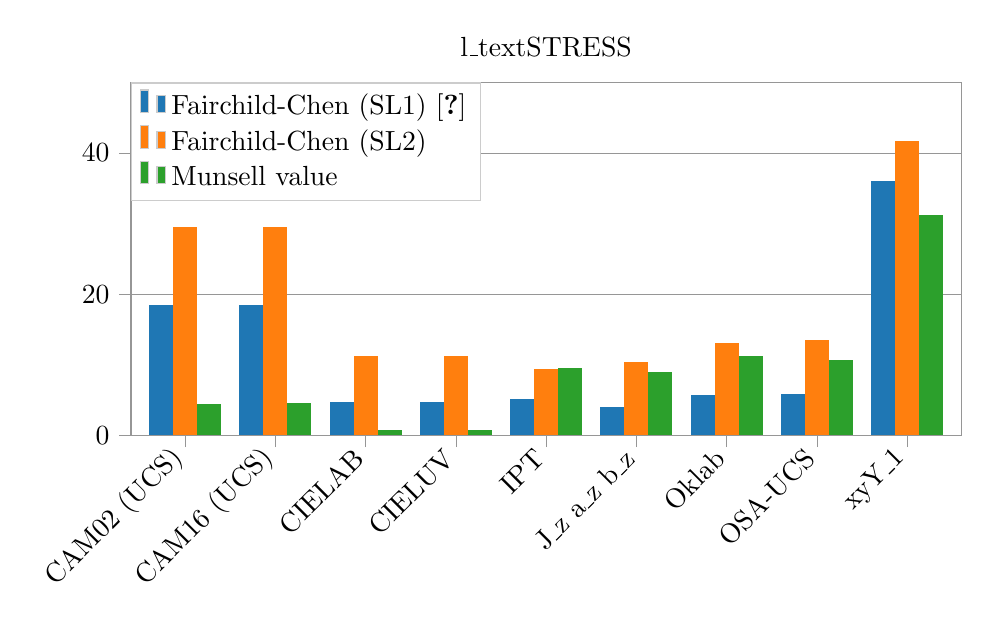
\begin{tikzpicture}

\definecolor{color0}{rgb}{0.12156862745098,0.466666666666667,0.705882352941177}
\definecolor{color1}{rgb}{1,0.498039215686275,0.0549019607843137}
\definecolor{color2}{rgb}{0.172549019607843,0.627450980392157,0.172549019607843}

\begin{axis}[
axis line style={white!58.8235294117647!black},
height=0.5\textwidth,
legend cell align={left},
legend style={
  fill opacity=1,
  draw opacity=1,
  text opacity=1,
  at={(0,1)},
  anchor=north west,
  draw=white!80!black
},
tick align=outside,
tick pos=left,
title={l\_{text{STRESS}}},
width=\textwidth,
x grid style={white!58.8235294117647!black},
xmin=-0.6, xmax=8.6,
xtick style={color=white!58.8235294117647!black},
xtick={0,1,2,3,4,5,6,7,8},
xticklabel style={rotate=45.0,anchor=east},
xticklabels={CAM02 (UCS),CAM16 (UCS),CIELAB,CIELUV,IPT,J\_z a\_z b\_z,Oklab,OSA-UCS,xyY\_1},
y grid style={white!58.8235294117647!black},
ymajorgrids,
ymin=0, ymax=50,
ytick style={color=white!58.8235294117647!black},
yticklabel style={anchor=east}
]
\draw[draw=none,fill=color0] (axis cs:-0.4,0) rectangle (axis cs:-0.133333333333333,18.4645911268359);
\addlegendimage{ybar,ybar legend,draw=none,fill=color0};
\addlegendentry{Fairchild-Chen (SL1) \cite{fairchildchen}}

\draw[draw=none,fill=color0] (axis cs:0.6,0) rectangle (axis cs:0.866666666666667,18.462147583011);
\draw[draw=none,fill=color0] (axis cs:1.6,0) rectangle (axis cs:1.86666666666667,4.67289145504149);
\draw[draw=none,fill=color0] (axis cs:2.6,0) rectangle (axis cs:2.86666666666667,4.67289145504149);
\draw[draw=none,fill=color0] (axis cs:3.6,0) rectangle (axis cs:3.86666666666667,5.16507600277125);
\draw[draw=none,fill=color0] (axis cs:4.6,0) rectangle (axis cs:4.86666666666667,4.0793287828234);
\draw[draw=none,fill=color0] (axis cs:5.6,0) rectangle (axis cs:5.86666666666667,5.64665508676546);
\draw[draw=none,fill=color0] (axis cs:6.6,0) rectangle (axis cs:6.86666666666667,5.82738652177515);
\draw[draw=none,fill=color0] (axis cs:7.6,0) rectangle (axis cs:7.86666666666667,35.9945312574285);
\draw[draw=none,fill=color1] (axis cs:-0.133333333333333,0) rectangle (axis cs:0.133333333333333,29.5046968567554);
\addlegendimage{ybar,ybar legend,draw=none,fill=color1};
\addlegendentry{Fairchild-Chen (SL2)}

\draw[draw=none,fill=color1] (axis cs:0.866666666666667,0) rectangle (axis cs:1.13333333333333,29.4786529029533);
\draw[draw=none,fill=color1] (axis cs:1.86666666666667,0) rectangle (axis cs:2.13333333333333,11.2665102417932);
\draw[draw=none,fill=color1] (axis cs:2.86666666666667,0) rectangle (axis cs:3.13333333333333,11.2665102417932);
\draw[draw=none,fill=color1] (axis cs:3.86666666666667,0) rectangle (axis cs:4.13333333333333,9.42833864558851);
\draw[draw=none,fill=color1] (axis cs:4.86666666666667,0) rectangle (axis cs:5.13333333333333,10.428911813808);
\draw[draw=none,fill=color1] (axis cs:5.86666666666667,0) rectangle (axis cs:6.13333333333333,13.1227691380623);
\draw[draw=none,fill=color1] (axis cs:6.86666666666667,0) rectangle (axis cs:7.13333333333333,13.4430812029788);
\draw[draw=none,fill=color1] (axis cs:7.86666666666667,0) rectangle (axis cs:8.13333333333333,41.6824228979887);
\draw[draw=none,fill=color2] (axis cs:0.133333333333333,0) rectangle (axis cs:0.4,4.37071391926707);
\addlegendimage{ybar,ybar legend,draw=none,fill=color2};
\addlegendentry{Munsell value}

\draw[draw=none,fill=color2] (axis cs:1.13333333333333,0) rectangle (axis cs:1.4,4.60456291212743);
\draw[draw=none,fill=color2] (axis cs:2.13333333333333,0) rectangle (axis cs:2.4,0.692826553107365);
\draw[draw=none,fill=color2] (axis cs:3.13333333333333,0) rectangle (axis cs:3.4,0.692826553107365);
\draw[draw=none,fill=color2] (axis cs:4.13333333333333,0) rectangle (axis cs:4.4,9.47504412245566);
\draw[draw=none,fill=color2] (axis cs:5.13333333333333,0) rectangle (axis cs:5.4,8.90523847167804);
\draw[draw=none,fill=color2] (axis cs:6.13333333333333,0) rectangle (axis cs:6.4,11.1924669875584);
\draw[draw=none,fill=color2] (axis cs:7.13333333333333,0) rectangle (axis cs:7.4,10.7060560056212);
\draw[draw=none,fill=color2] (axis cs:8.13333333333333,0) rectangle (axis cs:8.4,31.2517455700297);
\end{axis}

\end{tikzpicture}

  \caption{lightness stress.}
\end{figure}


\cite{munsell}
\cite{fairchildchen}

\section{Optimization}

It has become fashionable to propose a color space format with free parameters, and then
optimize those parameters against a number of goal functionals. Examples are
\cite{prolab,oklab,jzazbz}.


% \printbibliography{}
\bibliography{main}{}
\bibliographystyle{plain}

\end{document}
